\documentclass[11pt]{article}
\usepackage[T1]{fontenc}
\usepackage[utf8]{inputenc}
\usepackage{lmodern}
\usepackage[margin=0.82in]{geometry}
\usepackage{microtype}
\usepackage{amsmath,amssymb}
\usepackage{booktabs,tabularx,longtable,array}
\usepackage[dvipsnames]{xcolor}
\usepackage{enumitem,tikz,fancybox}
\usetikzlibrary{arrows.meta,positioning}
\usepackage{hyperref,fancyhdr,titlesec}

\definecolor{navy}{HTML}{17365D}
\definecolor{blue}{HTML}{2F75B5}
\definecolor{teal}{HTML}{218A8D}
\definecolor{lightblue}{HTML}{EAF3F8}
\definecolor{lightteal}{HTML}{EAF6F4}
\definecolor{warm}{HTML}{F8F1E7}
\definecolor{red}{HTML}{B13A3A}
\definecolor{graytext}{HTML}{4A5560}
\hypersetup{colorlinks=true,linkcolor=navy,citecolor=teal,urlcolor=blue,
  pdftitle={Adjoint-Faithful FNO for a Baroclinic Double Gyre}}
\pagestyle{fancy}\fancyhf{}
\lhead{Adjoint-faithful FNO}\rhead{Minimum-data project plan}\cfoot{\thepage}
\renewcommand{\headrulewidth}{0.3pt}
\setlength{\headheight}{14pt}
\titleformat{\section}{\Large\bfseries\color{navy}}{\thesection}{0.7em}{}
\titleformat{\subsection}{\large\bfseries\color{blue}}{\thesubsection}{0.7em}{}
\setlist[itemize]{leftmargin=1.35em,itemsep=2pt,topsep=4pt}
\setlist[enumerate]{leftmargin=1.55em,itemsep=2pt,topsep=4pt}
\setlength{\parindent}{0pt}\setlength{\parskip}{5pt}
\renewcommand{\arraystretch}{1.18}
\newcolumntype{Y}{>{\raggedright\arraybackslash}X}
\newcommand{\MITgcm}{\textsc{MITgcm}}
\newcommand{\AF}{AF--FNO}
\newsavebox{\decisionstore}
\newsavebox{\contractstore}
\newsavebox{\examplestore}
\newenvironment{decisionbox}
  {\begin{center}\begin{lrbox}{\decisionstore}\begin{minipage}{0.92\textwidth}}
  {\end{minipage}\end{lrbox}\setlength{\fboxsep}{8pt}%
   \fcolorbox{teal}{lightteal}{\usebox{\decisionstore}}\end{center}}
\newenvironment{contractbox}
  {\begin{center}\begin{lrbox}{\contractstore}\begin{minipage}{0.92\textwidth}}
  {\end{minipage}\end{lrbox}\setlength{\fboxsep}{8pt}%
   \fcolorbox{red}{warm}{\usebox{\contractstore}}\end{center}}
\newenvironment{examplebox}[1]
  {\begin{center}\begin{lrbox}{\examplestore}\begin{minipage}{0.92\textwidth}%
   \textbf{#1}\par\smallskip}
  {\end{minipage}\end{lrbox}\setlength{\fboxsep}{8pt}%
   \fcolorbox{blue}{lightblue}{\usebox{\examplestore}}\end{center}}

\begin{document}
\pagenumbering{gobble}
\begin{titlepage}
\centering\vspace*{0.9in}
{\sffamily\bfseries\color{navy}\fontsize{25}{30}\selectfont
Adjoint-Faithful Fourier Neural Operator\\[0.18in]
for a Baroclinic Double Gyre\par}
\vspace{0.3in}{\Large A minimum-data summer internship project plan\par}
\vspace{0.55in}
\begin{decisionbox}
\centering
\textbf{Core idea:} first establish a frozen, adapted Bire-architecture baseline on the
same \MITgcm{} trajectories used by \AF{}. Then improve the operator with modern
forward losses and a small set of forward perturbation--response pairs. Generate true
\MITgcm{} adjoints only after the emulators are frozen, and use them as a blind test.
\end{decisionbox}
\vfill
{\large Revised technical proposal --- 29 July 2026\par}\vspace{0.45in}
{\small Ten-week scope; official \MITgcm{} baroclinic-gyre tutorial;
NeuralOperator 2.0 implementation\par}
\end{titlepage}

\pagenumbering{roman}
\tableofcontents
\clearpage
\pagenumbering{arabic}

\section{Recommendation in one page}
\begin{decisionbox}
\textbf{Recommended path.} Build an \textbf{adjoint-faithful FNO (\AF)} on the official
\MITgcm{} baroclinic double-gyre tutorial at \(1^\circ\). Before changing the architecture
or loss, train a frozen \textbf{A0 adapted Bire FNO} on exactly the same trajectories.
This tests transfer of the paper's qualitative trends---useful short forecasts, stable
rollouts, and sensitivity to wind amplitude---without claiming a bitwise reproduction
of its undocumented \(0.25^\circ\) dataset. Then introduce the modern A--D ladder:
A and B are controlled baselines, C is selected for forward fidelity, and D adds
forward-only response supervision. Do not put a single \MITgcm{} adjoint in training or
model selection.
\end{decisionbox}

The minimum credible programme is:
\begin{itemize}
\item \textbf{Three long production regimes}: low, control, and high wind amplitude.
\item \textbf{Two short held-out wind runs}: the intermediate amplitudes used by
Bire et al.; inference-only and not 20 years long.
\item \textbf{One frozen architecture-transfer baseline (A0)}: the recovered Bire FNO
core, adapted only where the \(62\times62\), 46-state benchmark forces a change. It is
trained and evaluated before the modern A--D models.
\item \textbf{224 ten-day perturbed restarts}: 128 training, 32 validation, and 64
inference. They provide local tangent information from forward \MITgcm{} only and total
about \(6.1\) model-years.
\item \textbf{Twelve true-adjoint runs}: three smooth objectives, two horizons, and
two unseen initial states, opened only after the model and criteria are frozen.
\end{itemize}

This separates four questions: Does the Bire architecture transfer to the documented
tutorial data? Does modernization improve the forward emulator? Did response supervision
improve the local input--output map? Does automatic differentiation through it yield a
useful adjoint? The defensible claim is deliberately limited: \emph{adjoint fidelity over
specified horizons, objectives, states, and a tested control subspace}.

\begin{contractbox}
\textbf{No-adjoint-training contract.} \MITgcm{} adjoints are excluded from training,
hyperparameter tuning, early stopping, loss selection, perturbation-amplitude selection,
and architecture selection. The test is run only after checksums of the frozen model and
evaluation script are recorded.
\end{contractbox}

\section{Research question and hypotheses}
Let the \MITgcm{} time-\(\Delta t\) map be
\[
x_{n+1}=\mathcal{M}_{\Delta t}(x_n,u_n),
\]
where \(x\) is the state and \(u\) contains forcing and controls. The FNO
\(\mathcal{F}_\theta\) approximates the same map. For a scalar objective \(J(x_N)\),
\[
\lambda_n^{\mathrm{FNO}}=
\left(\frac{\partial\mathcal{F}_\theta}{\partial x_n}\right)^{T}
\lambda_{n+1}^{\mathrm{FNO}},\qquad \lambda_N=\nabla_{x_N}J.
\]

\textbf{Primary question.} Can local derivative information obtained exclusively from
short forward perturbation experiments make these gradients agree with \MITgcm{}
adjoints more closely than a state-accurate forward FNO?

\textbf{Hypotheses:} (1) the adapted A0 baseline reproduces the qualitative Bire forecast
and wind-response trends on the coarser tutorial; (2) a forward-selected modern FNO
improves forecast, rollout, boundary, and resolved-scale behavior relative to A0;
(3) state accuracy alone does not ensure adjoint accuracy; and (4) adding a local
response loss to a forward-credible model improves gradient direction without adjoint
labels or material loss of forward skill.

\section{Why local perturbation--response information is the right approach}
\subsection{A small state error can hide a wrong derivative}
Suppose \(\mathcal{M}(x)=x\), but an emulator learns
\[
\mathcal{F}(x)=x+\delta\sin(kx),\qquad
\mathcal{F}'(x)=1+\delta k\cos(kx).
\]
The state error never exceeds \(\delta\), yet the derivative error can be large when
\(k\) is large. A value-only loss controls the height of a learned curve at sampled
points; it does not adequately control its slope. An adjoint is built from those slopes.

\begin{examplebox}{Intuitive ocean example}
Two emulators predict sea-surface height ten days ahead to within one centimetre. In one,
a small extra wind-stress patch strengthens the western boundary current; in the other,
it weakens it. Their forecast scores can be almost identical, but a gradient-based
optimization steps in opposite directions. One perturbed forward run reveals the
physical response sign without computing an adjoint.
\end{examplebox}

\subsection{Forward responses teach Jacobian actions}
At an anchor \(z=(x,u)\) and normalized direction \(v\), run the model from \(z\) and
\(z+\varepsilon v\):
\[
r_M(z;v,\varepsilon)=
\frac{\mathcal{M}_{\Delta t}(z+\varepsilon v)-\mathcal{M}_{\Delta t}(z)}
{\varepsilon}\approx D\mathcal{M}_{\Delta t}(z)v .
\]
Match it with the emulator secant
\[
r_\theta(z;v,\varepsilon)=
\frac{\mathcal{F}_{\theta}(z+\varepsilon v)-\mathcal{F}_{\theta}(z)}
{\varepsilon}.
\]
This constrains a Jacobian--vector product (JVP) using only forward simulations and
ordinary first-order training backpropagation. The link to adjoints is duality:
\[
\underbrace{v^TD\mathcal{M}(z)^Tq}_{\text{gradient projected on }v}
=\underbrace{q^TD\mathcal{M}(z)v}_{\text{objective response along }v}.
\]
Thus, matching \(D\mathcal{M}v\) for relevant directions also matches projections of
adjoints for many later objectives \(q\). The full Jacobian remains too large to identify;
the claim must stay within the sampled smooth wind and state subspace.

\section{Benchmark choice: trend, not hidden dataset}
The public \texttt{oceanfourcast} repository is a conceptual starting point, not an exact
reproduction package. Its training defaults differ from the paper, its README points to
external data, and its loader predicts ten selected channels including diagnostic
pressure and streamfunction. Reimplement the method in the maintained NeuralOperator
library rather than preserve old dependencies \cite{OceanFourCast,NeuralOperator}.

\begin{table}[htbp]\centering\small
\caption{Published setup, official tutorial, and proposed benchmark.}
\label{tab:benchmarks}
\begin{tabularx}{\textwidth}{@{}p{0.19\textwidth}YYY@{}}
\toprule
& \textbf{Bire et al.} & \textbf{Official tutorial} & \textbf{Proposed} \\
\midrule
Grid & \(0.25^\circ\), \(248\times248\) & \(1^\circ\), \(60\times60\) ocean cells plus land border & Tutorial first; fine grid only as stretch \\
Vertical & 15 levels, about \(2\,\mathrm{km}\) & 15 levels, \(1.8\,\mathrm{km}\) & Tutorial levels \\
Time step & \(300\,\mathrm{s}\) & \(1200\,\mathrm{s}\) & Tutorial value \\
\(\tau_0\) (\(\mathrm{N\,m^{-2}}\)) & 0.075, 0.0875, 0.100, 0.1125, 0.125 & Default 0.100 & Same five amplitudes \\
Training winds & Low, control, high & Not applicable & Low, control, high \\
Held-out winds & Two intermediates & Not applicable & Same two; short runs \\
Goal & Forward emulation & Numerical tutorial & Forward and local-adjoint fidelity \\
\bottomrule
\end{tabularx}
\end{table}

This removes uncertainty about an unavailable initialization and pipeline, reduces the
horizontal cell count by about 16, and retains the relevant baroclinic physics. The
tutorial notes that the deep ocean is still adjusting after 100 years; stationarity must
therefore be measured for the variables and horizons used \cite{MITgcmTutorial}.

\subsection{A0: a time-boxed Bire-architecture transfer baseline}
Do not make the incomplete public repository a prerequisite for the project. Audit the
paper, repository, and recovered implementation once; record unresolved discrepancies;
then freeze A0 and label it \emph{adapted} rather than exact. Implement it through the
public NeuralOperator 2.0 \texttt{SpectralConv} interface while retaining the recovered
paper structure: channel-diagonal Fourier multipliers, explicit pointwise channel
mixing, three Fourier blocks, width 128, alternating sine/cosine position fields, and
paper-style one-step state loss and optimizer schedule.

All models must use the same S0--S2 source states, chronological splits, masks, and
training-only normalization. Only adaptations forced by the documented benchmark are
allowed in A0:

\begin{table}[htbp]\centering\small
\caption{Declared adaptations from the Bire configuration to A0.}
\label{tab:a0-adaptations}
\begin{tabularx}{\textwidth}{@{}p{0.23\textwidth}p{0.25\textwidth}Y@{}}
\toprule
\textbf{Element} & \textbf{Bire / recovered setting} & \textbf{A0 on the tutorial} \\
\midrule
Horizontal grid & \(248\times248\) at \(0.25^\circ\) & \(62\times62\) including the land rim \\
Dynamic state & Ten selected prognostic/diagnostic outputs & All 46 Markov-state channels; wind is the additional input \\
Fourier modes & \([64,64]\) & \([16,16]\), preserving the approximate mode-to-grid ratio \\
Coarse pretraining & Stride 8, yielding \(31\times31\) & Not used in the frozen A0; this is a recorded departure, not an inferred reproduction \\
Forecast target & Normalized next state & Retain for A0; Models A--D predict a normalized residual \\
Software & Historical \texttt{oceanfourcast} environment & Recovered architecture on pinned NeuralOperator 2.0 \\
\bottomrule
\end{tabularx}
\end{table}

Run a 20--100-sample overfit test, one ten-day development training, and the locked
low/control/high evaluation. Do not tune A0 after opening held-out I1/I2 results. If the
recovered baseline cannot learn the small sample after the declared learning-rate
fallbacks, report that result and proceed; repairing historical code must not delay the
\AF{} experiment. Separate five- and 30-day A0 models are optional follow-ups only when
needed to compare a specific Bire lead-time panel.

\section{Minimum MITgcm simulation programme}
\subsection{Five original trajectory jobs plus three authorized extensions}
\begin{table}[htbp]\centering\small
\caption{Minimum trajectories. Durations are planning budgets; diagnostics decide
whether equilibration is adequate.}
\label{tab:runs}
\begin{tabularx}{\textwidth}{@{}p{0.07\textwidth}p{0.10\textwidth}p{0.17\textwidth}p{0.19\textwidth}Yp{0.12\textwidth}@{}}
\toprule
\textbf{ID} & \(\boldsymbol{\tau_0}\) & \textbf{Duration} & \textbf{Initialization} & \textbf{Use} & \textbf{Output} \\
\midrule
S0 & 0.100 & 100 y spin-up; final 10 y production & Tutorial initial state & Control data; branch checkpoint & Annual restart; daily production \\
S1 & 0.075 & 5 y adjust + 10 y production & S0 checkpoint & Low-wind data & Daily production \\
S2 & 0.125 & 5 y adjust + 10 y production & S0 checkpoint & High-wind data & Daily production \\
E0 & 0.100 & 10 y extension & S0 year-110 pickup & Version-2 control coverage & Daily production \\
E1 & 0.075 & 10 y extension & S1 local year-15 pickup & Version-2 low-wind coverage & Daily production \\
E2 & 0.125 & 10 y extension & S2 local year-15 pickup & Version-2 high-wind coverage & Daily production \\
I1 & 0.0875 & 1 y & Unseen S0-derived state & Interpolation inference only & Daily \\
I2 & 0.1125 & 1 y & Different unseen state & Interpolation inference only & Daily \\
\midrule
\multicolumn{2}{@{}l}{\textbf{Total}} & \textbf{172 model-years} & \multicolumn{3}{l}{Original 142 plus 30 evidence-authorized extension years} \\
\bottomrule
\end{tabularx}
\end{table}

After year 50, inspect five-year trends of heat content, surface kinetic energy,
basin-integrated transport, and level-mean temperature. Stop at year 100 only if the
upper-ocean quantities are statistically stationary; otherwise extend the run or narrow
the first claim. The \(1^\circ\) grid and four-times-larger time step should be much
cheaper per model-year than Bire's setup, but wall-clock/model-year must be benchmarked.

\subsection{Chronological data splits}
Use years 1--7 for training, year 8 for validation, and years 9--10 for inference within
each ten-year S0--S2 production segment. Insert 90-day gaps at boundaries.

\begin{table}[htbp]\centering\small
\caption{Data roles. Pair counts are approximate for daily output and a ten-day target.}
\label{tab:splits}
\begin{tabularx}{\textwidth}{@{}p{0.20\textwidth}p{0.22\textwidth}p{0.16\textwidth}Y@{}}
\toprule
\textbf{Dataset} & \textbf{Source} & \textbf{Approx. size} & \textbf{Permitted use} \\
\midrule
Trajectory training & S0--S2 years 1--7 & 7,500 pairs & Fit weights \\
Trajectory validation & S0--S2 year 8 & 1,000 pairs & Tune and early-stop \\
Known-wind inference & S0--S2 years 9--10 & 2,100 pairs & Final scores only \\
Unseen-wind inference & I1 and I2 & 700 pairs & Final interpolation only \\
Response training & 16 anchors \(\times\) 8 directions & 128 endpoints & Fit response loss \\
Response validation & 4 anchors \(\times\) 8 directions & 32 endpoints & Tune loss and \(\varepsilon\) \\
Response inference & 4 anchors \(\times\) 8 directions \(\times\) 2 signs & 64 endpoints & Blind central differences \\
True adjoints & 3 costs \(\times\) 2 horizons \(\times\) 2 states & 12 integrations & Blind comparison only \\
\bottomrule
\end{tabularx}
\end{table}

The 224 perturbed restarts add 2,240 model-days, about \(6.1\) model-years. Save only
initial/final states, configuration hash, and perturbation definition. A 46-channel
\(62\times62\) float32 snapshot is about \(0.7\,\mathrm{MB}\); 30 daily production years are of
order \(8\,\mathrm{GB}\) before compression.

\subsection{Eight directions per response anchor}
\begin{table}[htbp]\centering\small
\caption{Minimum smooth perturbation basis.}
\label{tab:directions}
\begin{tabularx}{\textwidth}{@{}p{0.12\textwidth}p{0.27\textwidth}Y@{}}
\toprule
\textbf{Count} & \textbf{Direction family} & \textbf{Purpose} \\
\midrule
1 & Prescribed cosine-wind amplitude & Directly tests the Bire control axis \\
1 & Smooth meridional wind phase/shape mode & Separates amplitude from pattern learning \\
2 & Smooth localized wind envelopes & Probe western/southern and northern/interior control \\
4 & Balanced, low-wavenumber state directions & Training-only EOFs or filtered anomalies; rotate among anchors \\
\bottomrule
\end{tabularx}
\end{table}

Pilot standardized amplitudes \(10^{-3}\), \(3\times10^{-3}\), and \(10^{-2}\). Select
the largest for which a central-difference linearity check is within 5--10\%, then freeze
the rule by direction family. Use randomly signed one-sided perturbations for training
and central differences for the blind response test.

\section{State, forcing, and preprocessing}
\subsection{Predict a Markov state, not independent diagnostics}
Place the prognostic variables on a documented common tracer grid and stack vertical
levels as channels:
\[
x=[U_{1:15},V_{1:15},\Theta_{1:15},\eta],
\qquad C_{\mathrm{out}}=46.
\]
Vertical velocity, pressure, and streamfunction are not independent prognostic channels.
Streamfunction is diagnosed from all 15 U levels.  For the present z-coordinate,
linear-EOS, constant-salinity configuration, pressure is reconstructed as the exact
\MITgcm{} diagnostic \texttt{PHIHYD}, i.e.\ hydrostatic pressure anomaly divided by
\(\rho_0\), in \(\mathrm{m^2\,s^{-2}}\):
\[
\frac{\rho_k'}{\rho_0}=-\alpha_T(\Theta_k-T_{\mathrm{ref},k}),\qquad
\Phi_k'=g\eta+\mathcal{H}_k\!\left(\frac{\rho'}{\rho_0}\right).
\]
Here \(\mathcal{H}\) is the fixed finite-difference vertical integration implemented in
\texttt{calc\_phi\_hyd.F}; the \(g\eta\) term matches \texttt{diags\_phi\_hyd.F}.
Report \(\Phi'\) at Bire's zero-based surface, mid-depth, and bottom indices
\(0,7,14\).  Physical pressure anomaly in Pa is \(\rho_0\Phi'\).  This map is linear,
differentiable, and has a fixed transpose \(\mathcal{H}^T\) for later adjoint objectives.
It therefore adds evaluation views but no new learned information or output channels.
If salinity later becomes active and nonconstant, add its 15 levels and update the
equation of state rather than silently omitting it.

The implementation was checked against the archived S0 \MITgcm{} final-state
\texttt{PH} dump at iteration 2,851,200 over all 15 levels and 3,600 wet cells.
Maximum absolute error was \(3.89\times10^{-4}\ \mathrm{m^2\,s^{-2}}\) and RMSE was
\(9.75\times10^{-6}\ \mathrm{m^2\,s^{-2}}\), passing the predeclared
\(10^{-3}\) maximum-error tolerance.  The reproducible report is
\path{outputs/af_fno/pressure_validation_v1/pressure_validation.json}.

The barotropic circulation diagnostic has a different verification contract.  From
raw C-grid faces,
\[
U_{\rm bt}=\sum_k U_k\Delta z_k,\qquad
V_{\rm bt}=\sum_k V_k\Delta z_k,\qquad
\Psi_U=-\int U_{\rm bt}\,dy,\qquad
\Psi_V=\int V_{\rm bt}\,dx .
\]
The production output is explicitly the \emph{U-derived barotropic transport
streamfunction}, matching the tutorial construction.  A training-only audit uses one
fixed 360-day year from each S0--S2 regime and compares independent raw-face U and V
prefix integrals over daily and 5/30/90/360-day means.  Version 1 verified the project
centered-U operator exactly but also exposed that centering U and V paths onto north
and east faces creates a spurious 10.9\% comparison.  Corrected version-2 contract
SHA-256 \texttt{88ff2f20fe1a...dea170} retained the fixed year and thresholds and
collocated both paths at identical C-grid corner indices.  All regimes pass: daily
p90 relative mismatch is at most \(3.25\times10^{-5}\), daily mean absolute mismatch
is \(1.14\)--\(3.49\times10^{-4}\)~Sv, 360-day mismatch is
\(4.74\)--\(6.00\times10^{-5}\)~Sv, spatial correlation is effectively one, and all
outer-boundary normal transports are zero.  Artifacts are under
\path{outputs/af_fno/streamfunction_consistency_v2/}.

This is strong numerical path consistency, not the same algebraic statement as the
pressure reconstruction.  With the linear free surface,
\[
\partial_t\eta+\nabla_h\!\cdot\mathbf U_{\rm bt}=0,
\]
so an instantaneous daily field may retain a very small divergence when SSH changes.
Use the U-derived label for instantaneous products, allow the validated transport
streamfunction interpretation for daily and time-mean comparisons in this
configuration, and retain this caveat in figures and gates.

Inputs comprise the 46 dynamic channels, wind stress, and normalized longitude, latitude,
wet mask, and distance-to-wall fields. Record every C-grid interpolation operator.
Compare gradients only after applying the exact transpose of those operators so the FNO
and \MITgcm{} sensitivities share a native control basis.

Compute channel means and scales from trajectory training only, mask land, and store the
affine transform with the model. Gradient comparisons must undo normalization:
\[
\widetilde{x}_i=(x_i-\mu_i)/\sigma_i
\quad\Longrightarrow\quad
\frac{\partial J}{\partial x_i}
=\frac{1}{\sigma_i}\frac{\partial J}{\partial\widetilde{x}_i}.
\]
Models A--D predict the normalized ten-day residual
\(\Delta\widetilde{x}_n=\widetilde{x}_{n+1}-\widetilde{x}_n\). This gives the
network an explicit identity path and focuses capacity on change. A0 alone retains the
recovered paper-style normalized next-state target; this intentional difference belongs
to the architecture-transfer baseline and must be stated in every A0 comparison.

\section{Modern adjoint-faithful FNO}
\subsection{Starting implementation}
After freezing A0, use the maintained \texttt{neuraloperator} package and pin its release
and commit. Begin the common A--D ladder with a modest dense FNO:

\begin{table}[htbp]\centering\small
\caption{Starting \AF{} configuration. Validation uses only trajectories and forward
responses.}
\label{tab:fno}
\begin{tabularx}{\textwidth}{@{}p{0.27\textwidth}p{0.23\textwidth}Y@{}}
\toprule
\textbf{Choice} & \textbf{Starting value} & \textbf{Reason / limited search} \\
\midrule
Forecast interval & 10 days & Economical response runs; useful scale in Bire et al. \\
Fourier modes & \([16,16]\) & Compare 12, 16, 24 after inspecting spectra; respect Nyquist \\
Hidden channels & 32 & Increase to 64 only if a 20--100-sample overfit test fails \\
FNO layers & 4 & Current library default; compact enough for ablation \\
Local branch & \texttt{conv\_bias\_kernel=3} & Complements global mixing near boundaries \\
Boundary treatment & 10\% domain padding & Reduces periodic FFT wrap in a closed basin \\
Geometry & Grid embedding, mask, wall distance & Makes solid boundaries explicit \\
Channel MLP & Enabled & Mixes the vertical state channels locally \\
Precision & float32 & Avoid mixed precision in the initial derivative study \\
Factorization & Dense FNO first & TFNO is a memory fallback, not an initial confounder \\
\bottomrule
\end{tabularx}
\end{table}

Select mode count from the resolved power spectrum: too few modes oversmooth the western
boundary current; too many learn aliased fluctuations. Domain padding or Fourier
continuation is relevant because the basin is not periodic. These choices follow the
NeuralOperator 2.0 practical guide rather than the outdated oceanfourcast environment
\cite{Duruisseaux2026}.

\subsection{Baseline ladder and controlled losses}
For a one-step pair and response direction, use
\begin{align}
\mathcal{L}={}&\mathcal{L}_{\mathrm{state}}
+\lambda_{\mathrm{roll}}\mathcal{L}_{\mathrm{roll}}
+\lambda_{\mathrm{resp}}\mathcal{L}_{\mathrm{resp}}
+\lambda_{\mathrm{spec}}\mathcal{L}_{\mathrm{spec}}
+\lambda_{\mathrm{bnd}}\mathcal{L}_{\mathrm{bnd}},\\
\mathcal{L}_{\mathrm{resp}}={}&
\frac{\lVert W_r(r_\theta-r_M)\rVert_2^2}
{\lVert W_r r_M\rVert_2^2+\epsilon_0}.
\end{align}
\(\mathcal{L}_{\mathrm{state}}\) is masked relative \(L_2\);
\(\mathcal{L}_{\mathrm{roll}}\) is a three-step (30-day) unrolled loss;
\(\mathcal{L}_{\mathrm{spec}}\) compares binned spectra; and
\(\mathcal{L}_{\mathrm{bnd}}\) upweights wet cells near the western wall. An
\(H^1\)-style spatial loss may supplement the spectral term, but it is not a substitute
for \(\mathcal{L}_{\mathrm{resp}}\): spatial output derivatives and derivatives of the
input--output operator are different objects.

\begin{table}[htbp]\centering\small
\caption{Required architecture-transfer baseline and controlled model ladder.}
\label{tab:ablations}
\begin{tabularx}{\textwidth}{@{}p{0.07\textwidth}p{0.26\textwidth}YY@{}}
\toprule
\textbf{Model} & \textbf{Training signal} & \textbf{Purpose} & \textbf{Expected result} \\
\midrule
A0 & Adapted Bire architecture and paper-style one-step loss & Test architecture transfer before modernization & Qualitative Bire trend on the common data \\
A & Modern dense FNO + one-step residual state loss & Controlled modern baseline & Comparable state skill; derivatives may be poor \\
B & Model A + rollout + spectral/boundary losses & Isolate modern forward losses from response data & Better rollout and boundary state skill \\
C & Forward-selected dense FNO + balanced state/increment, rollout, tapered spectral, and boundary losses & Establish a forward-credible emulator before derivative training & Pass the complete forward gate \\
D & Frozen Model C design + local response loss & Test the \AF{} hypothesis without asking derivative data to repair the forward model & Preserve C's state skill; improve responses and adjoints \\
\bottomrule
\end{tabularx}
\end{table}

Models A and B remain frozen controls; B is not retroactively retuned.  Model C is the
only forward-selection stage, and its search is limited and recorded below.  Model D
copies only a Model C configuration that has passed its complete forward gate; rejected
validation-search v1 does not qualify.  It then preserves that configuration's
architecture, preprocessing, and forward objective and adds
\(\mathcal{L}_{\mathrm{resp}}\).  Increase \(\lambda_{\mathrm{resp}}\) only on response
validation data until response error improves without worsening C's validation state
error by more than 5\%.  Lock all weights before viewing any true adjoint.

\subsection{Model C: predeclared forward-selection protocol}

The preliminary A/B results show that architecture plausibility is not enough:
temperature and SSH can be worse than persistence even when the 46-channel aggregate
loss improves.  Following the practical FNO workflow in Duruisseaux et al.
\cite{Duruisseaux2026}, Model C therefore separates representation, optimization, and
data adequacy rather than changing all three at once.

\begin{decisionbox}
\textbf{Model C implementation contract opened 23 July 2026.}  The first implementation
retains the 51 declared raw inputs, NeuralOperator grid lifting, dense float32 spectral
weights, Channel MLP, four-layer width-32 starting point, 10\% padding, and parallel
\(3\times3\) local branch.  It replaces B's channel-aggregated objective with equal
U/V/temperature/SSH group terms, scales increment error with training-only per-channel
ten-day RMS, and compares spectra of increments on the exact \(60\times60\) wet
rectangle after a Hann taper.  Initial forward/backward checks contain 630,262
parameters at width 32 and 2,443,542 at width 64.  Width 64 is therefore a conditional
capacity test, not the assumed default.  Training-only C1a calibration subsequently
froze increment/rollout/spectral/boundary coefficients
\(0.001/0.15/10^{-5}/0.065\); these scales precede all validation and architecture
selection.
\end{decisionbox}

\begin{examplebox}{C0 training-only audit, 23 July 2026}
The sealed audit verified the dataset metadata hash and read only 7,530 training pairs.
The per-channel normalized ten-day increment RMS spans a factor of 147, so channelwise
increment scaling is necessary.  At \((16,16)\), the global Fourier path contains
8.8\%, 24.0\%, 67.8\%, and 85.6\% of tapered U, V, temperature, and SSH increment
energy; full-state fractions all exceed 99.6\%.  The local branch is therefore essential,
and more modes alone cannot represent most velocity-increment energy.  The
\((24,16)\) candidate captures 12.5\%/32.9\% for U/V, compared with
9.0\%/25.6\% for \((16,24)\); it was added before validation was opened.  Increment
autocorrelation implies only about 278--398 effective samples across the three regimes,
with S1 much more correlated than S0/S2.  This supports regime-balanced learning curves,
but not immediate replacement of version-1 data.
\end{examplebox}

\begin{examplebox}{C1a loss-gradient calibration, 23 July 2026}
Complex-safe CPU job 285116 completed in 4m39s using only the same 96 balanced training
rollouts.  After its 20-epoch core warmup, state/increment/rollout/spectral/boundary
gradient norms were 1.965/830.5/6.484/40,763/7.411.  The automatically clipped proposal
was rejected: coefficients 0.01 would still make increment and spectral gradients
dominate.  Unclipped targets were
\(0.001183/0.1515/1.205\times10^{-5}/0.06629\); the rounded frozen coefficients above
produce weighted gradient ratios 0.423/0.495/0.207/0.245 relative to state.  The very
small spectral coefficient does not remove spectral supervision because its raw
gradient is about 20,700 times the state gradient.  Pending GPU replica 284858 was
cancelled with zero runtime.  No candidate checkpoint or validation metric was produced.
\end{examplebox}

\begin{examplebox}{C1b--C1d memorization diagnosis, 23--26 July 2026}
Training-only job 285192 completed both controlled 160-epoch attempts in 58m30s.
At learning rate 0.001 it passed total, spectral, state-group, rollout, and boundary
criteria, but temperature/SSH increment errors were 1.802/2.888 times persistence on
the exact 96 records.  Learning rate 0.0005 improved these to 1.285/2.032; U/V were
already 0.254/0.442 times persistence.  Therefore C1b is rejected specifically for
slow-field increments despite a 97.7\% total reduction, 99.1\% spectral reduction,
0.0304 maximum state-group error, 0.0312 rollout, and 0.0397 boundary error.

The lower learning rate achieved its best total at the final epoch, so C1c job 285265
fixed the data, loss, architecture, seed, and batch order and extended 160 to 320
epochs.  At its epoch-315 minimum, U/V/temperature/SSH ratios were
0.206/0.353/0.979/1.219; all other criteria and exact reload passed.  Width-64 GPU job
285325 also completed 320 epochs but was rejected at 0.145/0.292/1.083/1.385 at its
selected epoch, and its best balanced SSH ratio was 1.302.  More duration and four
times the parameter count therefore did not remove the SSH failure.  Every evaluated
checkpoint and both rejected diagnostic checkpoints are retained; no validation data
were opened.
\end{examplebox}

\begin{examplebox}{Late-objective audit and accepted optimization schedule, 26 July 2026}
GPU array job 287581 independently rechecked all 64 evaluated epochs in each 320-epoch
history and differentiated the full 96-record mean loss at both late checkpoints.
Increment contributed only 5.7\% and 7.2\% as much value as state at widths 32 and 64,
but its weighted gradient norm was already 0.422 and 0.406 times the state gradient.
The increment gradient was dominated by SSH and aligned with state (cosines 0.966 and
0.927), while late SSH errors fluctuated strongly.  This evidence supports an
optimization diagnosis rather than another capacity increase.  Operational CPU
fallback job 287556 measured the same short width-64 workload in 436/272/253 seconds
at 4/8/16 cores; 16 cores is the measured fallback, while GPU remains primary and
backend replication is not a scientific priority.

Bounded array job 287583 then isolated two training-only changes.  Raising only the
increment coefficient from 0.001 to 0.0025 (loss v2) was rejected; its best balanced
SSH ratio remained 1.328.  Keeping loss v1 and reducing the learning rate once from
0.0005 to 0.0001 after epoch 240 passed the complete gate at epoch 315:
U/V/temperature/SSH were 0.211/0.360/0.794/0.990 times persistence, total/spectral
reductions were 98.24\%/99.82\%, maximum state-group error was 0.0248,
rollout/boundary were 0.0231/0.0301, and three-step reload was bitwise exact.
Only epoch 315 passed every group, so the result authorizes the bounded validation
search but is not itself a validated or frozen final Model C.
\end{examplebox}

\begin{decisionbox}
\textbf{Model C validation-search contract frozen before validation metrics, 26 July
2026.}  The machine-readable contract
\path{config/model_c_validation_search_v1.json} has SHA-256
\texttt{9e1d44299ae6...c4c6f6}.  It compares the five declared mode pairs at widths
32/64 and four layers/10\% padding in four from-scratch successive-halving rounds:
\(10\rightarrow5\rightarrow3\rightarrow2\rightarrow1\).  Chronology and optimizer
steps increase together as 25\%/1,920, 50\%/3,840, 75\%/5,760, and
100\%/7,680.  Every round decays learning rate 0.0005 to 0.0001 at 75\% of its
step budget; the full round exactly transfers the accepted 96-record schedule by
optimizer step rather than by dataset-dependent epoch count.

Eight predeclared checkpoint fractions are scored on all 780 ten-day validation pairs
and 16 fixed 180-day-capable starts per regime.  Ranking is lexicographic: require all
four physical-unit U/V/temperature/SSH RMSE ratios below persistence, minimize their
worst ratio, then minimize the arithmetic mean of full-domain, western-boundary, and
Hann-tapered local-increment spectral ratios at 30/90/180 days.  Search seed 20260723
is fixed.  The final architecture must then pass every ten-day group independently for
seeds 20260723/20260724/20260725 with exact reload before any inference data open.
Padding 20\% or six layers may be tested only for the two finalists and only under the
contract's explicit wall-leakage or training-underfit triggers; no combined variant is
allowed.  At contract freeze, only split metadata had been inspected---no validation
state metric, inference, intermediate-wind, response, or adjoint datum had been read.
\end{decisionbox}

\begin{examplebox}{Completed bounded validation search and three-seed decision,
26 July 2026}
GPU jobs 287604/288466/289379/289915 completed every candidate in the four
from-scratch \(10\rightarrow5\rightarrow3\rightarrow2\rightarrow1\) rounds.
Stage-manifest SHA-256 values are \texttt{40b54530d7d9...12d2f05},
\texttt{a2d639f8940c...d5e382}, \texttt{9bbd4fc4ce3c...f30e17}, and
\texttt{453c05ec408f...2fea2}.  The selected full-resource architecture was
\((24,16)\), width 64, four layers, and 10\% padding.  Its
U/V/temperature/SSH validation ratios were
0.1473/0.3547/0.6597/1.00014, with physics score 22.84; the other finalist,
\((16,24)\), width 64, gave 0.1577/0.3723/0.6353/1.02477 and 28.22.
Training worst-group ratios 0.915/0.941 and boundary/full-domain ratios
0.667/0.639 left both predeclared conditional triggers false, so neither six layers nor
20\% padding was tested.

Final-seed GPU array 290382 then retrained the selected architecture from scratch for
seeds 20260723/20260724/20260725.  All jobs completed with scheduler exit zero, matching
source/data/normalizer contracts, sealed later-data flags, and bitwise-exact three-step
reload.  Every seed beat persistence for U, V, and temperature, but SSH ratios were
1.00014/1.00383/1.03818.  The frozen rule is strict, so the immutable decision records
\texttt{scientifically\_rejected\_three\_seed\_gate},
\texttt{configuration\_frozen=false}, and
\texttt{inference\_authorized=false}.  Decision SHA-256 is
\texttt{e19d502442fc...72155}; internal freeze-contract SHA-256 is
\texttt{a44622cee685...73628}.  The full-domain mean group ratio also grows from
0.704--0.765 at 30 days to 3.21--3.45 at 90 days and 53.54--61.90 at 180 days.
Therefore validation-search v1 is scientifically rejected, not rounded into a
near-threshold pass, and no inference or response/adjoint archive opens.
\end{examplebox}

The following list preserves the prospectively declared protocol that produced this
decision; it is not authority to continue tuning after the v1 rejection.

\begin{enumerate}
\item \textbf{Training-only diagnostics.}  Compute tapered two-dimensional spectra of
  normalized states and ten-day increments by variable group, verify padding and
  mode indexing, run a stronger 96-sample memorization test, and log both raw and
  weighted loss terms and their gradient norms.  Report U, V, temperature, and SSH
  separately; the 15/15/15/1 channel multiplicity must not decide the fit.
\item \textbf{Repair the objective before enlarging the network.}  Start from B's dense
  four-layer, width-32 architecture.  Use an equal-weight mean of the four
  group-normalized state errors, add a group-balanced normalized-increment error, retain
  the three-step rollout, and compute spectral loss after wet-field extension and a
  fixed taper so the land discontinuity is not mistaken for unresolved physics.
  Normalize boundary and spectral terms by group and choose their weights from the
  training diagnostics, then freeze the weights for candidate comparison.
\item \textbf{Small representation search.}  Compare mode pairs
  \((12,12),(16,16),(16,24),(24,16),(24,24)\) and widths 32 and 64 with four layers and
  10\% padding.  Use successive halving on fixed training/validation blocks.  For only
  the two best candidates, test padding 20\% and six layers if the failure diagnostic
  specifically indicates wall leakage or insufficient capacity.  Dense float32
  spectral weights, lifting, projection, Channel MLP, mask, wall distance, and the local
  \(3\times3\) branch remain mandatory; factorization is a memory fallback.
\item \textbf{Freeze by validation, then test once.}  Train the selected configuration
  with three fixed seeds.  Candidate ranking is lexicographic: first require every
  U/V/temperature/SSH ten-day validation RMSE ratio to beat persistence; next minimize
  the worst group ratio; then minimize the predeclared mean of 30-, 90-, and 180-day
  rollout, boundary, and resolved-spectrum scores.  Inference years, I1/I2, response
  inference, and adjoints remain sealed until the configuration, seeds, code, and
  normalizer hashes are recorded.  The complete 10--360-day package is run only after
  that freeze.
\end{enumerate}

This search is deliberately not ``try until a test plot looks good.''  A candidate that
reduces the aggregate validation loss but remains worse than persistence for any state
group is not selected.  Conversely, increasing Fourier modes is not automatic: the
62-point grid limits meaningful frequencies, and added modes are accepted only when
training-only increment spectra and held validation metrics support them.
For the real-valued NeuralOperator convolution, a declared
\(\texttt{n\_modes}=(m_y,m_x)\) retains \(m_y\) centered Fourier rows but only
\(m_x/2+1\) nonnegative real-FFT columns internally.  Every spectral audit and report
uses that exact convention rather than interpreting \(16\times16\) as 256 independent
complex coefficients.

\textbf{Calibration backend rule.}  CUDA is an efficiency choice, not a scientific
requirement for the C1a loss-gradient calibration.  Its 20 epochs on 96 training
rollouts completed on eight CPU cores in 4m39s.
The CPU and GPU replicas must use the same data, records, seed, architecture, and loss
code but write separate artifacts.  If both complete, compare raw terms, gradient
ordering, and proposed weighted contributions; modest floating-point differences are
expected, whereas an order-of-magnitude disagreement blocks the loss freeze and requires
diagnosis.  Global gradient norms are accumulated in float64 for real gradients and
complex128 for complex spectral-weight gradients even though model arithmetic remains
float32/complex64; this prevents diagnostic overflow without discarding the imaginary
component.  Neither backend output is a candidate checkpoint or validation result.

\subsection{Data-adequacy and expansion gate}

The existing version-1 trajectories are sufficient to diagnose and select Model C:
across S0--S2 they provide 7,530 overlapping ten-day training pairs, 780 validation
pairs, and 1,860 sealed inference pairs.  They are not 7,530 independent realizations,
because adjacent daily pairs overlap strongly.  More consecutive years would therefore
increase the raw count much faster than the effective sample size.

Before generating replacement data, run learning curves on chronological 25, 50, 75,
and 100\% subsets, estimate integral autocorrelation times for the four state groups,
compare training and validation error by group, and measure the three-seed spread.
The evidence is considered \emph{data-limited} only when a candidate can fit the training
blocks, validation skill improves consistently with more chronology, and between-seed
or between-regime generalization remains the dominant error.  Poor training fit or
insensitivity to added chronology points instead to optimization, capacity, or the
objective and does not authorize more \MITgcm{} years.

\begin{examplebox}{Post-search data-adequacy decision, 27 July 2026}
The selected \((24,16)\), width-64 candidate fits the full training chronology
(worst-group ratios 0.915--0.928 across the three final seeds), while its validation
worst-group ratio improves monotonically with chronological coverage:
2.168, 1.483, 1.192, and 1.00014 at 25/50/75/100\%.  The three final SSH ratios span
1.00014--1.03818.  Contract
\path{config/model_c_data_adequacy_v1.json}, SHA-256
\texttt{e185301947b4...53c84a9}, was frozen before per-regime checkpoint metrics.
GPU job 290415 passed all four rules.  Temperature/SSH state-RMS effective sample totals
are only 7.59/7.69; S0, S1, and S2 all have positive median validation--training SSH
gaps.  Aggregate SSH block-bootstrap intervals include persistence.

The audit also prevents a data-only interpretation.  Median S1 SSH ratios are 1.354 on
training and 1.508 on validation, while S0/S2 are below persistence.  Thus
\texttt{trajectories\_v2} is authorized, but the low-wind objective/capacity imbalance
and long-rollout instability must still be addressed prospectively.
\end{examplebox}

Expansion contract \path{config/trajectories_v2_expansion.json}, SHA-256
\texttt{7ee2ae10330a...fe045ed}, adds ten exact, continuous production years to each
immutable S0--S2 endpoint in a new
\path{mitgcm_v2/} root.  Exact continuation is chosen over an artificial pickup
perturbation so the added states remain on precisely the same forced attractors and the
record length approaches the reference study.  Raw coverage doubles, but effective
coverage is recomputed after conversion and is not assumed to double automatically.
Version 1 and every conclusion based on it remain immutable.

The 7,200-record-per-regime successor split contains two seven-year training blocks,
the original sealed inference block, and fresh validation/inference blocks separated by
90-day buffers.  The already-open v1 validation block is excluded from successor
selection.  This yields 15,060 training pairs, 780 fresh validation pairs, and 3,450
sealed inference pairs across S0--S2.

\begin{examplebox}{Trajectory-v2 completion and coverage gate, 27 July 2026}
Array job 290439 completed the three exact continuations in 15m10s--15m31s.  Each
produced 3,600 daily \texttt{dynState}/\texttt{surfState} records, the endpoint pickup,
and a normal \MITgcm{} termination.  Build job 290443 created the 11~GB
\path{trajectories_v2.zarr} store with shape
\(3\times7200\times46\times62\times62\).  Independent job 290444 verified finite
states, zero land values, exact daily iteration spacing, a bitwise-identical v1 prefix,
bitwise raw-MDS extension samples at days 1/1800/3600, and independently reproduced
training-only normalizers.  Dataset metadata and quality-report SHA-256 values are
\texttt{ae7be47c4569...78b8cc} and \texttt{a6f7e5234ace...cf752}.

Coverage contract \path{config/trajectories_v2_coverage_audit.json}, SHA-256
\texttt{e539ca1bb61a...9197f36}, was frozen only after quality validation and before
coverage metrics.  Training-only job 290446 then measured temperature/SSH state-RMS
effective multipliers of 2.142/2.039 and ten-day-increment multipliers of 2.106/2.253.
Thus the predeclared two-times slow-field target passed.  The velocity state proxies are
not used for this decision because some per-regime integral-time estimates are much
less stable between the two decades.  Report SHA-256:
\texttt{7758cfb64e73...18e5}.
\end{examplebox}

Successor-training contract\newline
\path{config/model_c_successor_training_v1.json}, SHA-256
\texttt{3e0a300e73ec...159285}, was frozen before reading any v2 training metric.
It holds loss v1, \((24,16)\) modes, four layers, 10\% padding, seed, optimizer
exposure, and split-1 records fixed.  Phase 1 compares the exact selected width-64
architecture on v2 with a width-64 candidate changing only Channel-MLP expansion from
\(0.5C\) to Bire's \(4C\).  Phase 2 restores width 128, lift/projection width 256, and
\(4C\) mixing only after both phase-1 reports complete.  A prospective training gate
requires every U/V/temperature/SSH group in every regime to beat persistence, exact
three-step reload, finite 180-day rollout, and normalized state-amplitude ratios in
\([0.5,2]\) at 90 and 180 days.  Both tasks in GPU array 290448 completed with exit
zero, exact reload, finite rollouts, and every amplitude check passing.  The data-only
control failed only S1 SSH at 1.103435 times persistence over all 5,020 S1 training
pairs.  Isolated \(4C\) channel mixing reduced that ratio to 1.003573 and improved the
aggregate U/V/temperature/SSH ratios by 23.6/22.2/9.4/7.9\%, but still fails the exact
unrounded gate.  Contracted phase-2 job 290597 then completed normally in 1h20m22s.
Width 128 passes the complete gate: its aggregate U/V/temperature/SSH ratios are
0.049040/0.121279/0.384816/0.522413, every regime/group is below persistence, and
S1 SSH is 0.762683.  Exact reload, finite 180-day rollout, and every amplitude check
also pass.  Report/checkpoint SHA-256 values are
\texttt{5946515ea81a...68433c}/\texttt{2d10e48adc5e...360060}; lightweight phase
results are preserved under \path{outputs/af_fno/C/successor_training_v1/}.
This all-group rule is deliberately a training-capacity diagnosis: a dense 46-output
model should be able to fit every supervised group.  It is not the final validation
metric and does not restore SSH as the sole forward-model veto.
Width 128 restores the reference's absolute latent, lift/projection, and Channel-MLP
widths, but its latent-to-output ratio is still only \(128/46=2.78\), versus
\(128/10=12.8\) for Bire.  A failure would therefore keep group-specific projection or
barotropic auxiliary structure scientifically motivated; it would not justify an
unbounded width search.

Fresh-validation contract:
\begin{quote}
\path{config/model_c_successor_validation_v2.json}\\
SHA-256 \texttt{56bb6ec59799...0cf27b}.
\end{quote}

It was frozen before any split-2 state metric.  It declares seeds 20260723, 20260724,
and 20260725 and scores every complete 10--90-day start.  Surface speed, SST, and
derived surface pressure are primary fields.  Persistence, training climatology, and
A0 are baselines.  The contract also fixes paired regime-stratified block bootstrap
and mandatory SSH and streamfunction stability.  Contract v1 is preserved but
superseded: a metadata-only
audit found 180 rather than 181 complete starts per regime (indices 6300--6479);
no validation state was read and no scientific criterion changed.  GPU array 290673
completed the two missing seeds on split 1.  All three seeds pass every prospective
training criterion, with worst regime/group ratios
0.762683/0.732270/0.839507, exact reload, and finite amplitude-bounded 180-day
rollouts.  Frozen fresh-validation GPU job 290738 completed operationally but rejected
the configuration scientifically.  Surface speed passes every comparison; the
three-seed bootstrap-mean SST/surface-pressure RMSE-AUC ratios to persistence are
2.313/2.198.  Their mean day-10 ratios are 0.861/0.578 but errors cross persistence
around days 20--30 and reach 4.862/4.636 by day 90.  This is an autoregressive
slow-field failure, not an SSH-only or one-step-capacity failure.

All seeds remain finite, preserve zero land, and pass SSH/streamfunction amplitude and
wind-slope checks.  The normalized-maximum ceiling 20 is exceeded at
21.169--21.367, but validation truth reaches 21.092; that subgate is
non-discriminating and the primary metrics independently reject the model.  Contract
\path{config/model_c_rollout_diagnosis_v1.json}, SHA-256
\texttt{d0ecee0db2b2...ff7ba}, froze a balanced 10--90-day split-1 audit before
any new architecture or loss decision.  GPU job 291102 completed in 3m58s with exit
zero and every seed reproduced good day-10 slow-field skill followed by failed
RMSE-AUC and day-90 skill.  Three-seed mean day-10/AUC/day-90 ratios to persistence
are 0.809/2.021/4.221 for SST, 0.552/1.867/3.873 for surface pressure, and
0.532/1.844/3.835 for SSH.  Apply the predeclared classification:
\texttt{training\_objective\_or\_checkpoint\_gate\_mismatch}.  This is not merely a
validation-only generalization gap and does not justify more \MITgcm{} data.
Intermediate winds I1/I2 and inference/perturbation/adjoint truth remain sealed.

Five project-facing validation figures are preserved under
\path{outputs/af_fno/C/successor_validation_v1/fresh_validation/}.  Their manifest
content SHA-256 is \texttt{8b24b6af0686...a0845f}; it binds each PNG to the immutable
report/array hashes.  Three further training-diagnosis figures, a lightweight summary,
and a manifest are under \path{outputs/af_fno/C/rollout_diagnosis_v1/}; diagnosis
manifest content SHA-256 is \texttt{664e66a0866d...393671}.  Neither plotting step read
a later archive.

\paragraph{Completed checkpoint, duration, and truncated-unroll audits.}
The practical guidance in Duruisseaux et al.\ \cite{Duruisseaux2026} points to the
observed mechanism directly.  Pages 62--64 distinguish easy, data-efficient one-step
autoregression from its long-horizon distribution shift: training sees true states,
whereas inference recursively consumes imperfect predictions and compounds error.
Recommended mitigations include short unrolled objectives, pushforward-style training,
noise/denoising, contractive behavior, and long-horizon statistical checks.  Pages
53--59 also warn against changing learning schedules, normalization, modes, and
capacity without first separating optimization, preprocessing, and representation;
pages 70--71 note that multi-objective gradients can be badly imbalanced.

Accordingly, another mode/width/data search was not started.  The frozen audit
contract was:
\begin{quote}
\path{config/model_c_checkpoint_replay_audit_v1.json}\\
SHA-256 \texttt{494ce9de6688...06682}.
\end{quote}
Job 291164 replayed the accepted seed-20260723 training exactly.  Architecture, loss v1,
optimizer, batch order, seed, and 15,360-step exposure are unchanged.  Save the six original late steps
11,520, 13,440, 14,400, 14,880, 15,120, and 15,360; require bitwise equality with the
hash-pinned step-14,880 state dictionary and zero numerical difference in the original
six-row training history.  Score each on the same 540 balanced split-1 starts at days
10--90.

A checkpoint-only correction was admissible only if one exact replay remained finite
and land-zero, retains the old every-regime/every-group ten-day gate, beats both
persistence and training climatology in 10--90-day RMSE-AUC for surface speed, SST,
and surface \(P/\rho\), and keeps SST/\(P/\rho\) below both baselines at every lead.
The replay completed in 1h19m14s.  Step 14,880 is bitwise exact and the original
six-row training history has zero numerical difference.  No checkpoint passes.
Diagnostic best step 14,400 retains ten-day skill but has worst primary RMSE-AUC
ratio 2.366 and worst slow-field lead ratio 5.513.  Therefore apply the frozen
\texttt{objective\_correction\_required} branch.

The first bounded correction is now frozen before training metrics:
\begin{quote}
\path{config/model_c_pushforward_objective_v1.json}\\
SHA-256 \texttt{406ee5248fb4...bccc2}.
\end{quote}
Starting from exact checkpoint 14,400, it preserves the architecture, normalization,
and every loss-v1 term.  It adds equal, climatology-scaled SST and surface-\(P/\rho\)
RMSE at alternating day-60/day-90 endpoints.  Intermediate recursive states are
detached and only the terminal ten-day map receives the auxiliary gradient; this
targets inference-state distribution shift with four backpropagated calls per batch
rather than a full nine-step graph.  The fixed coefficient \(0.0025\) makes the
initial auxiliary contribution comparable to the existing total.

GPU job 291612 completed 1,920 fine-tune steps and evaluated steps
480/960/1,440/1,920 on the same 540 split-1 rollouts.  A pass required primary
10--90-day RMSE-AUC below both baselines, SST and surface \(P/\rho\) below both at
every lead, the old ten-day regime/group gate, finite rollouts, zero land, and exact
reload.  Step 1,920 is best by every frozen priority and improves worst primary AUC
from 2.366 to 1.692 and worst slow-field lead ratio from 5.513 to 3.994, but the
gate remains failed.  It is not replicated and fresh validation remains closed.

The training-window total and both auxiliary terms decrease at every checkpoint, and
the stabilized \(2\times10^{-5}\) rate was active only for the final 480 steps.
Before changing the loss again, freeze:
\begin{quote}
\path{config/model_c_pushforward_duration_v1.json}\\
SHA-256 \texttt{4867fa77d68e...78c79}.
\end{quote}
This duration diagnosis replayed the complete 1,920-step path from checkpoint 14,400
with the identical seed, batch order, optimizer, objective, and decay at step 1,440.
The replayed step-1,920 state must match the completed job bit for bit before any
extension metric is trusted.  It then adds 3,840 steps at the already-decayed rate
and scores eight checkpoints from total step 2,400 through 5,760 on the same gate.
GPU job 291616 completed in 51m31s and the step-1,920 replay is bitwise exact.  None
of the eight duration checkpoints passes.  Diagnostic-best step 5,760 has worst
primary RMSE-AUC/slow-field lead ratios 1.597/3.609; at day 90, SST is
2.402/3.609 and surface \(P/\rho\) is 2.922/1.727 times
persistence/climatology.  Further low-rate exposure improves the curves but is not
sufficient.  Apply the predeclared classification that one-step terminal supervision
is structurally insufficient; do not replicate or validate this checkpoint.

The one authorized structural correction is now frozen before its metrics in
operationally corrected version 2:
\begin{quote}
\path{config/model_c_truncated_unroll_objective_v2.json}\\
SHA-256 \texttt{0c5aabadbe51...92e3c}.
\end{quote}
It begins at duration step 5,760 and retains width 128, modes \((24,16)\), four
layers, padding, normalization, loss-v1, the split-1 chronology, batch order,
climatology scales, coefficient \(0.0025\), and the complete 540-record gate.
The sole scientific change is gradient horizon.  Alternating batches supervise
three consecutive endpoints at days 40/50/60 or 70/80/90 and backpropagate through
all three ten-day calls; states before the selected window remain detached.  This is
short truncated backpropagation rather than a full nine-call graph, and directly
tests whether the learned operator can control recursive slow-field amplification.

Initial job 291769 stopped before training or scientific metrics because the source
validator expected \texttt{fine\_tune\_step}, whereas the duration checkpoint records
\texttt{total\_fine\_tune\_step}.  Version 2 changes no objective or data read: it
moves the corrected schema check into preflight.  Four focused tests, lint, shell
validation, all source hashes, and the training-only sealed-data preflight passed.
GPU job 291778 completed normally in 20m01s.  All four checkpoints remain finite and
land-zero, and diagnostic-best truncated step 1,920 reloads a nine-call rollout
bitwise exactly.  It fails every scientific gate.  Worst primary RMSE-AUC/slow-lead
ratios are 1.933/3.701, worse than the duration source's 1.597/3.609.  Its SST AUC
ratios to persistence/climatology are 1.479/1.933 and its surface-\(P/\rho\) ratios
are 1.298/0.585; day-90 values are 2.463/3.701 and 2.844/1.681.  SST first loses
persistence at day 30 and surface pressure at day 60.  The completed test therefore
rejects short three-call truncation as sufficient and does not authorize replicas or
fresh validation.  Report/arrays SHA-256 values are
\texttt{86f7981e7a0a...b5b830}/\texttt{0c5222cd6938...d716}; the project-facing
figure/CSV/summary are under
\path{outputs/af_fno/C/truncated_unroll_objective_v2/}.

\paragraph{Completed signed-bias diagnosis and completed loss-v3 objective.}
The evidence now supports slow-field tendency drift more strongly than a general
forecast failure.  Velocity and the transport streamfunction remain accurate, while
SST, SSH, and surface pressure start skillful and then accumulate error against an
almost stationary truth.  Pure capacity, loss-weight, duration, detached-pushforward,
and three-call-gradient variants are exhausted.  The training-only frozen-checkpoint
audit was
\begin{quote}
\path{config/model_c_slow_field_bias_projection_v1.json}\\
SHA-256 \texttt{fd7d39f5c6a4...05428}; job 292064.
\end{quote}
It uses every split-1 teacher-forced pair to measure the signed physical ten-day
increment error for SST, SSH, and all 15 temperature levels.  Nine times each
regime-specific bias field is compared with the reference seed's mean day-90 error on
the exact 540 starts used by job 291102, using area-weighted pattern correlation,
fixed-amplitude explained energy, basin mean, and a basin-mean-plus-five-increment-EOF
projection.  No checkpoint weight changes.

The same contract applies five post-hoc maps after every frozen model call: raw,
zero-wet-area-mean SSH increment, SSH plus per-level temperature-mean conservation,
static signed-bias subtraction, and static-bias subtraction plus both constraints.
SSH uses cosine-latitude wet-area volume weights.  Temperature targets the
regime-specific, per-level mean truth tendency measured only on split 1.  A
training-only scalar AR(1) baseline toward pointwise climatology and 10--720-day
SST/SSH anomaly correlations quantify whether persistence is already near the
deterministic limit.

Job 292064 completed in 7m09s without opening a held state.  Fixed-amplitude
\(9\epsilon\) explains 33.43\% of pooled day-90 SST error energy and 27.21\% of SSH,
below the predeclared 50\% bias-dominance criterion.  Basin mean plus the first five
training-increment EOFs explain only 4.57\%/1.73\% of SST/SSH day-90 error energy.
Static-bias subtraction plus conservation nevertheless reduces the worst slow-field
RMSE-AUC ratio from 1.986 to 1.603, a material 19.25\% improvement but just below the
frozen 20\% alternate threshold; conservation alone changes it to 1.996.  Apply the
declared \texttt{feedback\_amplification} branch:
static bias is real but not the dominant low-dimensional error, so forecast-age
conditioning is primary.  The four figures, CSV, and summary are preserved under
\begin{quote}
\path{outputs/af_fno/C/slow_field_bias_projection_v1/}.
\end{quote}
Immutable report SHA-256 is \texttt{e66b263c826c...0f90}; arrays SHA-256 is
\texttt{4e7f73c2384e...8547}.

The completed training contract is
\begin{quote}
\path{config/model_c_rollout_conditioned_loss_v3.json}\\
SHA-256 \texttt{37f1157851ac...5a08}.
\end{quote}
It starts from diagnostic-best duration step 5,760, preserves the width-128
one-state architecture, loss-v1 core, split-1 chronology, and 540-record gate, and
adds three attributable components.  Every model call is followed by the linear
zero-area-mean SSH projection and regime/level training-mean temperature-tendency
projection.  A weight-0.01 per-wet-cell batch-mean signed-increment penalty makes the
remaining temperature/SSH bias visible.  A weight-0.0025 auxiliary loss cycles over
days 10--90; all preceding projected forecast states are detached and exactly one
call from the selected forecast age receives this gradient.  Thus each update has
four differentiable calls---the three-call loss-v1 core plus one conditioned call---
without changing the eventual Model-D state interface.  Six checkpoints over 2,880
steps at \(2\times10^{-5}\) are scored before any replica or held-state read.

GPU job 292293 completed normally in 27m46s and opened no held state.  The selected
diagnostic checkpoint is loss-v3 step 960 and reloads nine calls bitwise.  Exact
projection residuals remain below \(3.73\times10^{-11}\) for normalized
area-mean SSH increment and \(1.17\times10^{-10}\) for normalized
temperature-mean tendency.  All four ten-day groups beat persistence, with aggregate
U/V/temperature/SSH ratios 0.0382/0.1058/0.2746/0.3456.  The strict 10--90-day gate
nevertheless fails: SST RMSE-AUC is 1.119/1.462 and surface-\(P/\rho\) is
1.364/0.615 times persistence/climatology; their day-90 ratios are
2.419/3.634 and 3.019/1.785.  Worst primary AUC improves from the duration
source's 1.597 to 1.462, but worst slow-field lead changes from 3.609 to 3.634.
Thus the constraints and forecast-age term improve the primary curve without
controlling terminal drift sufficiently; no replica, fresh validation, or automatic
loss/capacity variant is authorized.  Report/arrays/checkpoint SHA-256 values are
\texttt{e9af34326c36...7ba11}/\texttt{522fe6145735...edff}/
\texttt{e9f962878cb5...970b}.  The two project-facing plots, complete CSV, summary,
and hash manifest are under
\path{outputs/af_fno/C/rollout_conditioned_loss_v3/}.

\paragraph{Bire-derived state correction.}
The archive comparison identifies a difference in state representation more consequential
than another layer, mode, or padding change.  Bire centres and scales each channel at
each grid point over training time and predicts the normalized future state directly.
The present Model C instead uses one scalar mean/scale per channel and predicts a small
residual increment.  Its slow fields therefore occupy poorly conditioned nearly
identity coordinates: a small systematic feedback error is inexpensive at one call but
accumulates at every recursive call.

The primary representation contract is frozen before its training or validation
metrics:
\begin{quote}
\path{config/model_c_anomaly_direct_v1.json}\\
SHA-256 \texttt{fa38b41578f5...8acea}.
\end{quote}
It computes one wind-independent pointwise mean and population standard deviation from
all 15,120 split-1 S0--S2 snapshots.  Pooling regimes keeps the normalization smooth
with respect to wind amplitude for the later derivative study.  Each channel's wet
point scale is floored at its fifth percentile, with a \(10^{-6}\) absolute guard.
This changes exactly 5\% of wet points per channel; a floor equal to 1\% of the old
scalar scale was rejected during preflight because it would floor 69\% of SST points.
The exact mean, raw-scale, and floored-scale SHA-256 values are
\texttt{36489318e23f...a649}, \texttt{ca1cb352d25b...93d7}, and
\texttt{b08f340a70f1...a83f}.

The FNO output is the next pointwise-normalized anomaly state; it is never added to the
current state.  A zero dynamic output therefore maps to the pooled pointwise training
climatology.  Width 128, four blocks, modes \((24,16)\), 10\% padding, lift/projection
width 256, the \(4C\) Channel MLP, local \(3\times3\) branch, loss-v1 three-step core,
optimizer, seed, and batch order remain fixed.  Seven checkpoints from steps
3,840--15,360 are selected only on the same 540 balanced split-1 rollouts and strict
10--90-day gate.  After that selection, the same prospectively fixed 15 S2 members are
characterized through day 200.  The required deliverable is
\begin{quote}
\path{outputs/af_fno/C/anomaly_direct_v1/}\\
\path{model_c_bire_figure4_dt10_rmse_0_200_days.png},
\end{quote}
along with normalization, checkpoint-selection, training-curve, streamfunction, and
unclipped full-range plots.  LayerNorm/dropout, a three-block/no-padding control, and
group-specific heads remain subsequent bounded tests rather than simultaneous changes.
Eight focused and inherited figure tests, lint, shell validation, source hashes,
normalizer preflight, and a production-grid three-step differentiable smoke test pass.
Inference, intermediate-wind, response, and adjoint states remain sealed.

\textbf{Completed representation result, 28 July 2026.}  V100 job 303447 completed
normally in 1h29m32s and selected optimizer step 14,400 using split 1 only.  Its
strict training-only gate passes: the worst primary RMSE-AUC ratio to either baseline
is 0.394 and the worst SST/surface-\(P/\rho\) single-lead ratio is 0.519.  Aggregate
ten-day U/V/temperature/SSH ratios to persistence are
0.0820/0.1905/0.2345/0.2645.  On the prospectively fixed S2 members, 10--90-day
surface-speed/SST/surface-\(P/\rho\) RMSE-AUC ratios to persistence are
0.222/0.206/0.601; the corresponding ratios to climatology are
0.313/0.258/0.214.  At day 200 their RMSEs remain bounded at
0.00212~\(\mathrm{m\,s^{-1}}\), 0.0288~\({}^{\circ}\mathrm{C}\), and
0.0552~\(\mathrm{m^2\,s^{-2}}\), compared with the loss-v3 map's approximate
0.058, 4.50, and 3.13.  Surface pressure no longer runs away, although its day-200
error is 2.18 times the exceptionally small persistence error; it remains 0.768
times climatology.  The requested Figure~4 and all five companion plots are saved
under the contracted project output root.

This is evidence for the combined representation change, not yet a claim that every
random seed or the complete 360-day physical gate passes.  Before changing layers,
padding, regularization, or heads, the independent-seed contract
\begin{quote}
\path{config/model_c_anomaly_direct_replication_v1.json}\\
SHA-256 \texttt{dd7e0f92ef50...d8325f}
\end{quote}
freezes replicas 20260724/20260725.  Only initialization and seed-driven batch order
may change.  Each checkpoint is again selected on split 1 before repeating the
already fixed 15-member S2 characterization.

\textbf{Completed replication result, 29 July 2026.}  Array 303640 completed both
tasks normally, and all three seeds pass every frozen gate.  Their mean six-ratio
ranking scores are 0.30227, 0.24717, and 0.23184 for
20260723/20260724/20260725, so the predeclared median is seed 20260724 at step
13,440.  Its day-200 speed/SST/surface-\(P/\rho\) RMSE is
0.00242/0.0262/0.0223, below both persistence and climatology.  The sealed summary,
CSV, manifest, and comparison plot are under
\path{outputs/af_fno/C/anomaly_direct_replication_v1/}.

The complete held-inference contract was frozen before opening split 3:
\begin{quote}
\path{config/model_c_anomaly_direct_forward_v1.json}\\
SHA-256 \texttt{d11029fce3aa...c2f6c}.
\end{quote}
It fixes 45 starts wholly inside the fresh trajectory-v2 inference block, 36 ten-day
calls, the median checkpoint, persistence, regime climatology, training-only damped
persistence, and A0 on identical starts.  The separate adjoint-readiness gate requires
all three primary fields at days 10 and 30 to beat every baseline with positive ACC;
the long gate adds 10--90-day AUC, day-360 boundedness/drift, resolved spectra, and
wind-response slope.  The forcing-switch sign remains reported but non-vetoing until
matching \MITgcm{} truth exists.  This job may open only the declared inference states;
intermediate-wind, response, and adjoint archives remain sealed.

\textbf{Completed held-inference result, 29 July 2026.}  V100 job 303993
completed normally in 3m00s.  The separate 10/30-day adjoint-readiness
determination passes every primary-field comparison.  At day 30 the model
RMSE for surface speed, SST, and surface-\(P/\rho\) is
0.000781~\(\mathrm{m\,s^{-1}}\), 0.00798~\({}^{\circ}\mathrm{C}\), and
0.00524~\(\mathrm{m^2\,s^{-2}}\), with ACC
0.9767/0.9778/0.9977; each is below persistence, climatology, damped
persistence, and same-start A0.  The primary 10--90-day RMSE-AUC also beats
all four baselines.  The one-year rollout is finite, exactly zero on land, and
bounded at a maximum normalized magnitude of 15.81; final U/V/temperature/SSH
mean biases are only 0.00676/0.00306/0.000285/0.00653 training standard
deviations.  The streamfunction wind-slope ratio is 1.180 and the provisional
forcing-switch sign is correct.

The combined gate nevertheless remains a frozen \emph{failure}.  Five of seven
day-360 spectral ratios pass, but the modewise medians for mid-depth and bottom
\texttt{PHIHYD} are 22.29 and 9.63, above the factor-four bound.  Consequently
the complete adjoint campaign remains closed even though the short-horizon
scientific determination is retained as a pass.  The complete metrics, arrays,
scorecard, readiness plot, spectra, maps, snapshots, and stability figures are
under
\path{outputs/af_fno/C/anomaly_direct_forward_v1/}.

The immutable posthoc diagnosis
\path{outputs/af_fno/C/anomaly_direct_forward_spectral_diagnosis_v1/}
does not reinterpret that failure.  It shows that total integrated day-360
energy is 1.029 times truth at mid-depth and 0.947 at the bottom, while modes
\(k\geq10\) contain only 0.0159\% and 0.0193\% of the respective model energy
(truth shares \(2.24\times10^{-6}\) and \(5.26\times10^{-6}\)).  Thus the
failure is a real but small high-wavenumber tail rather than basin-scale drift
or an unstable attractor.  Before changing weights, the training-only
attribution contract
\begin{quote}
\path{config/model_c_anomaly_direct_training_spectral_attribution_v1.json}\\
SHA-256 \texttt{afb64d5a0f3a...d0246}
\end{quote}
fixes all three accepted seeds, 36 split-1 starts, all 15 pressure levels, and
360-day rollouts.  It will establish seed consistency, depth, and onset without
reading validation, inference, response, or adjoint state; only a
seed-consistent split-1 tail authorizes one prospective spectral-regularization
fine-tune.

\textbf{Rejected attribution implementation, 29 July 2026.}  Job 304125
completed normally in 1m07s, but its scientific output is invalid.  The runner
advanced the model by one ten-day call while gathering truth at daily offset
\(t+s\), not \(t+10s\).  The impossible 10--90-day primary RMSE ratios
3.48--4.48 times persistence exposed the mismatch.  Its output is retained only
as rejected provenance and cannot authorize a loss change.  The corrected
contract
\begin{quote}
\path{config/model_c_anomaly_direct_training_spectral_attribution_v2.json}\\
SHA-256 \texttt{29c344310e50...a3de1}
\end{quote}
pins a stride of ten daily snapshots per model call, verifies the inclusive
\(t\) through \(t+360\) window stays wholly in split 1, and replaces the
invalid starts with 12 fixed admissible times.  Six focused tests, lint, shell
validation, source hashes, and production-data preflight pass.  No
regularization or later archive read is authorized until this corrected
attribution completes.  V100 job 304177 completed normally in 1m11s and
validly classifies a seed-consistent training-split tail.  Across seeds
20260723--20260725, day-360 mid-level ratios are 12.25--13.54 and bottom ratios
are 4.96--5.69; failure begins at days 170--190 and 310--330, respectively.
Total mid/bottom pressure energy remains 1.02--1.07 times truth, while every
10--90-day primary ratio remains only 0.19--0.37 times persistence.  Report
content SHA-256 is \texttt{f3cb1bd6de11...141927}, and the immutable package is
under
\path{outputs/af_fno/C/anomaly_direct_training_spectral_attribution_v2/}.

\textbf{Single authorized spectral fine-tune, 29 July 2026.}  Contract
\begin{quote}
\path{config/model_c_anomaly_direct_deep_pressure_spectral_regularization_v1.json}\\
SHA-256 \texttt{4f3377382dc0...acef37}
\end{quote}
starts from median seed 20260724 at step 13,440 and changes only one term: a
weight \(10^{-3}\) differentiable complex-Fourier PHIHYD error over levels
7--14 and radial modes 10--30 on the existing 10/20/30-day rollout.  It fixes
1,920 constant-\(2\times10^{-5}\) fine-tune steps and five checkpoints.  The
same 36 corrected split-1 records select a candidate only if both mid and
bottom spectra stay within factor four at every lead through day 360, total
energy remains 0.8--1.25 times truth, every primary remains better than
persistence, and no primary degrades more than 10\% from the source.  Four
focused tests, lint, shell validation, source locks, and production-data
preflight pass.  V100 job 304324 completed normally in 10m25s.  The term
substantially helps but does not pass the prospective rule: at fine-tune step
1,920 the day-360 mid/bottom ratios fall from 13.37/5.57 to 6.19/2.97, the
bottom tail never crosses four, and mid-tail onset moves from day 180 to day
280.  Integrated mid/bottom energy remains 1.006/0.980 times truth and all
primary 10--90-day ratios improve or remain protected.  Because the mid-level
ratio still exceeds four, no fine-tune checkpoint is promoted; the selected
model remains original seed 20260724 at step 13,440.  Report/manifest content
SHA-256 is \texttt{8065faafeecf...ddb75}/
\texttt{280a863a5892...f3a8}, with JSON, arrays, and two plots under
\path{outputs/af_fno/C/anomaly_direct_deep_pressure_spectral_regularization_v1/}.
No second spectral weight or duration is authorized, and validation and later
archives remain sealed.

\textbf{Bire regularization factorial, 29 July 2026.}  Contract
\begin{quote}
\path{config/model_c_anomaly_direct_bire_regularization_controls_v1.json}\\
SHA-256 \texttt{dd9089e9675a...0f827}
\end{quote}
implements the next originally ordered Bire-derived control without extending
the failed spectral loss.  Three from-scratch seed-20260724 arms isolate
pointwise channel LayerNorm after spectral and Channel-MLP mixing, archived
Channel-MLP dropout 0.5, and their interaction.  The unregularized
seed-20260724/step-13,440 model is the fixed reference.  Every arm retains the
pointwise anomaly/direct-state representation, width 128, four layers,
modes \(24\times16\), padding 0.1, loss v1, data order, optimizer, and
15,360-step budget.  Seven checkpoints per arm are scored only on the corrected
36-member split-1 protocol through day 360 with the same factor-four,
integrated-energy, persistence, and 10\%-degradation guards.  Four focused
tests, lint, shell validation, all-arm production preflight, and finite
62-by-62 forward smoke tests pass.  No validation, held-inference, long-term,
response, or adjoint state may be read.  V100 array 304376 is submitted with
task mapping 0=LayerNorm, 1=dropout, and 2=combined.

\textbf{Bire long-term skill and learned-physics scope.}  A replicated
candidate must still undergo a Bire-section-5.3-style approximately 2,000-day
ensemble test.  Beyond decorrelation this is a bounded statistical test of
climatological mean and variance, drift, spatial spectra/scales, and mean
circulation, not a claim of trajectory RMSE superiority.  A Bire-section-6
learned-physics test is also required: initial-state and changed-wind
sensitivity must have the correct sign, amplitude, spatial pattern, and time
evolution.  The existing one-year boundedness and scalar wind-slope checks are
promising precursors, not substitutes.  Spatial response and forward/adjoint
archives remain sealed until the original combined forward gate passes.

\paragraph{Temporal-interface decision.}
The active Model C is one-input/one-output in \emph{time}, despite its
51 input and 46 output \emph{channel} counts.  Each call receives one 46-channel
state together with wind stress, longitude, latitude, mask, and wall distance, then
predicts one 46-channel ten-day residual.  Three-step autoregressive training exposes
the model to its own predictions but does not provide two past states to one call or
produce two future states directly.

Samudra instead used consecutive ocean states to predict two later states, arguing that
the pair supplies tendency-like context; Bire identified this two-time-step input/output
design as a future forecast-horizon comparison rather than using it in the reported
FNO.  It remains a bounded secondary arm rather than the next automatic job: the
streamfunction phase is already accurate through day 90, job 292064 selected the
forecast-age branch, and completed job 292293 improved primary AUC without passing
the long gate.  A later parameter/compute-accounted two-input/two-output temporal
ablation must retain the same data, Fourier modes, spatial trunk, conservation
projections, bias penalty, and prospective gate.  The latter
would naturally use 97 external inputs (two
46-channel states plus five forcing/static fields) and 92 dynamic outputs, and would
make the eventual Model D/adjoint state carry two consecutive ocean states.  Its extra
temporal context may reduce recursive phase error, but its larger interface and
paired-output consistency are costs, so improvement cannot be assumed from Samudra's
different global-OM4 ConvNeXt-UNet setting.

\paragraph{Bire-style presentation characterization.}
Bire Figure~3 shows barotropic streamfunction truth, prediction, and
truth-minus-prediction at days 0--40, followed by additional coarse-resolution rows;
Figure~4 shows mean RMSE with 10th--90th percentile shading over 15 randomly chosen
members.  Its persistence repeats each initial condition at all later leads.  Its
climatology is described as the pointwise time mean of the \MITgcm{} simulation, but
the article does not explicitly state whether evaluation times are excluded from that
mean.

Contract \path{config/model_c_bire_figures_v1.json}, SHA-256
\texttt{791c84f12c2d...eb696b}, is frozen before any 100--200-day validation metric.
It reproduces those definitions without opening inference: one hash-pinned
seed-20260723 checkpoint, 15 prospectively sampled S2 fresh-validation starts, and the
first prospectively drawn member for the spatial panels.  Figure~3 retains only the
native \(1^\circ\) truth/prediction/difference rows.  Figure~4 retains only
\(\Delta t=10\) days and fixes 0--200 days, red/black/blue
prediction/climatology/persistence curves, member mean and 10th--90th percentiles,
and requested limits 0--\(1.2\times10^{-1}\ \mathrm{m\,s^{-1}}\) for speed,
0--\(3\times10^{-1}\ ^\circ\mathrm{C}\) for SST, and
0--\(1\ \mathrm{m^2\,s^{-2}}\) for \(P/\rho\).  The climatology is the
regime-specific pointwise mean over all 5,040 split-1 training snapshots, with
nonlinear derived fields averaged after derivation.  This is a leakage-free
implementation of the paper's formula.  The output is descriptive evidence for the
already rejected model and cannot select a checkpoint, alter a loss/architecture, or
authorize inference.  GPU job 291134 completed normally in 51 seconds.  For the
prospectively selected S2 member, streamfunction RMSE at days 10/20/30/40 is
0.0316/0.0934/0.1580/0.1765~Sv against a truth RMS near 13.34~Sv.  Thus the
short-horizon circulation fields are very close; the shared paper-style
streamfunction scale makes the difference row intentionally faint.

All 15 predictions remain finite through day 200, but the long-horizon curves expose
severe recursive drift.  At day 200, Model-C/persistence RMSE is
0.07344/0.00480~\(\mathrm{m\,s^{-1}}\) for surface speed,
5.981/0.0505~\({}^{\circ}\mathrm{C}\) for SST, and
3.747/0.0253~\(\mathrm{m^2\,s^{-2}}\) for surface pressure.  Model mean SST
first exceeds its requested 0.3-degree axis at day 100, and surface pressure first
exceeds its requested \(1\ \mathrm{m^2\,s^{-2}}\) axis at day 160; speed remains
inside its requested axis.  Preserve this clipping because it is part of the requested
paper-matched presentation, and use the numerical archive for the off-scale values.
Report/arrays SHA-256 values are
\texttt{b704b921444d...e300ac5}/\texttt{a73ac9bf2cc9...20b1}; the two PNGs,
lightweight summary, and manifest-content SHA-256
\texttt{258be6fabe13...827f} are preserved under
\path{outputs/af_fno/C/bire_figures_v1/}.  Inference remains sealed.

Because the requested fixed axes visually compress the baselines, preserve that
paper-matched figure and add, rather than replace it with, the hash-pinned companion
\path{outputs/af_fno/C/bire_baseline_zoom_v1/}.  It reads only the immutable Figure-4
arrays and gives full-range plus baseline-scale SST and surface-\(P/\rho\) panels and
a complete CSV.  SST first exceeds both persistence and climatology at day 20.
Surface \(P/\rho\) first exceeds persistence at day 30 and climatology at day 70.
Contract/manifest-content SHA-256 values are
\texttt{2a2324090b83...b2a4a}/\texttt{01433936e406...99063}; the figure/CSV SHA-256
values are \texttt{1f1ea2c6f76a...6643f}/\texttt{542e74c02b59...068ce}.  This
addendum evaluates no model, changes no result, and opens no data.

To expose the visually small streamfunction errors without changing the completed
package, freeze the separate contract
\path{config/model_c_bire_streamfunction_leads_v1.json} before evaluating the
additional spatial maps.  Its SHA-256 is
\texttt{ccb965e58bdc...ae1934c}.
It fixes exactly eight new native-\(1^\circ\) figures at days 20, 30, \ldots, 90
for the same S2 start 6335 and hash-pinned checkpoint.  Each image contains
\MITgcm{} truth, Model C, and truth-minus-prediction.  Truth and prediction use one
common symmetric scale across all leads; each difference uses its own labeled
symmetric maximum-error scale and prints RMSE and maximum error.  This makes spatial
structure visible, but colors in different error panels must be interpreted through
their printed scales rather than compared directly.  Day 10 remains represented in
the original Figure-3 analogue.  The new immutable roots are
\path{/bigscratch/mjalabert314/bire_james25_repro/af_fno/models/C/bire_streamfunction_leads_v1/}
and \path{outputs/af_fno/C/bire_streamfunction_leads_v1/}.  This is descriptive
use of the already opened S2 validation member; inference and every later archive
remain sealed.

GPU job 291135 completed this contract normally in 35 seconds.  Streamfunction RMSE
increases from 0.0934~Sv, or 0.700\% of truth RMS, at day 20 to 0.2951~Sv, or
2.211\%, at day 90; maximum pointwise error increases from 0.7240 to 1.1713~Sv.
Thus the large-scale barotropic circulation remains visually close through day 90
even though the independently measured SST and surface-pressure trajectories drift
badly.  This variable-specific contrast strengthens the objective/checkpoint-mismatch
diagnosis: the entire spatial dynamics have not collapsed uniformly.  Preserve
report/arrays SHA-256 values
\texttt{71c6e1dc1f9a...89c206}/\texttt{b4126494d9c0...3bcd48} and all eight
hash-bound PNGs under the project output root; manifest-content SHA-256 is
\texttt{3b74d759d551...450ac7}.  The repeated days 20--40 agree with the original
package to FP32 roundoff, and no inference data were opened.

\begin{figure}[htbp]\centering
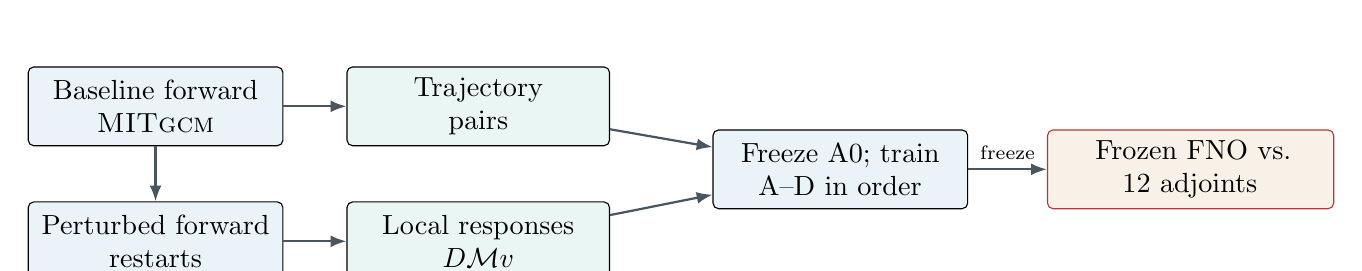
\begin{tikzpicture}[
node distance=7mm and 8mm,
box/.style={draw,rounded corners=2pt,align=center,minimum height=10mm,
  text width=30mm,fill=lightblue},
dat/.style={draw,rounded corners=2pt,align=center,minimum height=10mm,
  text width=31mm,fill=lightteal},
test/.style={draw=red,rounded corners=2pt,align=center,minimum height=10mm,
  text width=34mm,fill=warm},
arr/.style={-{Latex[length=2mm]},thick,draw=graytext}]
\node[box] (base) {Baseline forward\\\MITgcm{}};
\node[box,below=of base] (pert) {Perturbed forward\\restarts};
\node[dat,right=of base] (traj) {Trajectory\\pairs};
\node[dat,right=of pert] (resp) {Local responses\\\(D\mathcal{M}v\)};
\node[box,right=13mm of traj,yshift=-8mm] (fno) {Freeze A0; train\\A--D in order};
\node[test,right=10mm of fno] (adj) {Frozen FNO vs.\\12 adjoints};
\draw[arr] (base)--(traj);\draw[arr] (base)--(pert);
\draw[arr] (pert)--(resp);\draw[arr] (traj)--(fno);
\draw[arr] (resp)--(fno);\draw[arr] (fno)--node[above,font=\scriptsize]{freeze}(adj);
\end{tikzpicture}
\\[-1mm]{\small\color{red}The adjoint archive has no path into training or tuning.}
\caption{The common trajectory pipeline feeds A0 and A--D; response data enter only D,
and the adjoint evaluation remains sealed.}
\label{fig:flow}
\end{figure}

\section{Ground-truth MITgcm adjoint suite}
\subsection{Minimum: twelve integrations}
One adjoint integration returns sensitivities to the full initial state and active
controls for one scalar objective. It is therefore more efficient to vary objective,
horizon, and state than to run an adjoint for every perturbation direction.

\begin{table}[htbp]\centering\small
\caption{Blind matrix: \(3\) objectives \(\times\) \(2\) horizons \(\times\)
\(2\) initial states \(=12\) adjoint integrations.}
\label{tab:adjoints}
\begin{tabularx}{\textwidth}{@{}p{0.25\textwidth}Yp{0.17\textwidth}p{0.16\textwidth}@{}}
\toprule
\textbf{Smooth scalar objective} & \textbf{Reason} & \textbf{Horizons} & \textbf{States} \\
\midrule
Gaussian interior sea-surface-height average & Broad low-wavenumber response away from walls & 10, 30 days & Two unseen dates \\
Smooth western-boundary sea-surface-height average & Energetic region where spectral/boundary errors matter & 10, 30 days & Same dates \\
Area-weighted barotropic gyre-strength functional & Dynamical circulation measure; avoids nondifferentiable maxima & 10, 30 days & Same dates \\
\bottomrule
\end{tabularx}
\end{table}

Select dates and masks before opening any adjoint result; place dates at least 90 days
from split boundaries and one another. If mandatory tests succeed, an optional six-run
extension adds 90-day horizons. Before accepting a reference adjoint, run a Taylor
remainder or central directional finite-difference check at one test state per objective
family. This verifies \MITgcm{} but may not alter the emulator.

\subsection{Metrics and an operational test}
For gradients \(g_M\) and \(g_F\), report
\[
\mathrm{cosine}=\frac{g_F^Tg_M}{\lVert g_F\rVert_2\lVert g_M\rVert_2},
\quad
\mathrm{angle}=\cos^{-1}(\mathrm{cosine}),
\quad
\mathrm{relative\ error}=\frac{\lVert g_F-g_M\rVert_2}{\lVert g_M\rVert_2}.
\]
Convert both gradients to the same physical units and grid with explicit area/volume
weights. Report full-state scores and projections onto the directions in
Table~\ref{tab:directions}. Direction is primary: optimization can tolerate imperfect
magnitude but not a gradient pointing uphill. Also show signed maps, vertical profiles,
wavenumber spectra, and sign agreement in the largest-sensitivity region.

Finally, use the emulator gradient to propose a small control update, choose the step from
a predeclared short line search, and evaluate the objective with one forward \MITgcm{}
run. This tests usefulness without turning adjoints into labels.

\section{Evaluation and predeclared success criteria}
\subsection{Bire et al. as a qualitative forward benchmark}

The numerical errors in Bire et al. cannot be transferred to this experiment: their
$0.25^\circ$, more turbulent double gyre has $248\times248$ points and different state
variables, while the present tutorial has $62\times62$ points.  We instead predeclare
the following \emph{trends} from their complete forward study as the benchmark
\cite{Bire2025}:
\begin{enumerate}
\item Their ten-day map gave the best overall compromise among 5-, 10-, and 30-day
  maps.  It beat persistence and pointwise time-mean climatology at useful short leads;
  velocity lost deterministic skill first, near roughly three months, while pressure
  and surface temperature retained useful skill longer.
\item Spatial error grew first in the energetic western-boundary region.  At day 60
  the ten-day map retained the most credible large-scale and boundary structure; after
  deterministic phase information was lost, stable long integrations still retained
  the characteristic anomaly length scales.
\item The learned integrations remained bounded for thousands of model days.  The
  five-day map developed excessive low-wind mesoscale variability, whereas the
  30-day map aliased or missed propagating variability whose period was close to the
  map interval.  This makes spectra and longitude--time diagrams necessary alongside
  scalar RMSE.
\item Long-run maximum streamfunction increased approximately linearly with wind-stress
  amplitude, close to the expected Sverdrup trend for the ten-day map.  The low- and
  high-intermediate wind cases were held out of training, so their ordering was a real
  interpolation test rather than a fit diagnostic.
\item Their emulator did \emph{not} reliably steer from an initial condition from one
  regime after an abrupt change in imposed wind.  Initial-condition dynamics dominated
  the new forcing.  We record this negative result explicitly: matching the equilibrium
  wind ordering is necessary, but a response/adjoint model intended for control should
  also improve the forcing-switch response.
\end{enumerate}

``Reproduce or improve Bire's trends'' below means recover this evidence pattern, not
match their plotted values or claim an exact reproduction.  A model may decorrelate---a
chaotic forecast should---but it must beat both simple baselines before decorrelation,
remain bounded, preserve resolved spatial scales, and express the correct forcing
ordering.  The complete adjoint campaign does not open until at least one modern
forward model passes the gate below.

\subsection{Frozen forward evaluation package}

Evaluate A0 and Models A--D on identical chronological records and identical 15-member
ensembles in each forcing regime.  A0 is frozen before I1/I2 are opened and no model is
tuned after viewing response or adjoint tests.  Persistence and a regime-specific,
training-only pointwise mean are the two primary baselines.  The current configuration
has no imposed seasonal cycle, so calling the latter a daily climatology would be
misleading; a day-of-year climatology will be added only if seasonal forcing is added.

Every frozen model must produce the following versioned package.  Evaluation contract
version 2 adds the deterministic pressure postprocessor; version-1 packages remain
historical pre-pressure evidence and are never overwritten.  Machine-readable
JSON stores definitions, scalar summaries, start indices, hashes, and gate outcomes;
compressed NPZ stores the plotted arrays so a figure can be regenerated without rerunning
the network.
\begin{enumerate}
\item \textbf{Deterministic skill:} physical-unit RMSE and pointwise-climatology ACC from
  10 to 360 days for U, V, temperature, SSH, surface speed, SST, \texttt{PHIHYD} at
  levels 0, 7, and 14, and the U-derived barotropic transport streamfunction.  Curves show ensemble mean and 10--90\% range for the model,
  persistence, and climatology.  Report the first lead at which each method loses ACC
  or baseline skill; never infer stability from the ten-day score alone.
\item \textbf{Spatial failures:} common-scale truth/forecast/error snapshots and spatial
  RMSE maps at 10, 60, 180, and 360 days for all seven Bire-facing diagnostics:
  surface speed, SST, SSH, the three pressure levels, and the U-derived barotropic
  transport streamfunction.
  Report the first four wet cells from the western wall separately,
  plus full-domain vertical RMSE profiles, to expose boundary and deep-ocean drift.
\item \textbf{Stability and scale retention:} one-year trajectories of a surface
  kinetic-energy proxy, temperature, SSH, and maximum streamfunction; finite-value and land-mask
  checks; normalized mean/variance drift by depth; radially binned spectra for all seven
  Bire-facing diagnostics at 10, 90, 180, and 360 days; and a fixed-control-member SSH longitude--time diagram.  Spectra
  are interpreted only over bins with non-negligible truth energy.
\item \textbf{Forcing physics:} low/control/high curves of maximum streamfunction,
  surface speed, SST, and SSH, with model and \MITgcm{} slopes computed on the same
  ensemble.  Once generated, I1/I2 are added as inference-only interpolation points.
  A separate forcing-switch experiment initializes every branch from the same control
  states and changes only the prescribed wind; it is clearly labeled as a response
  diagnostic until matching switched-wind \MITgcm{} trajectories exist.
\item \textbf{Audit trail:} checkpoint and dataset hashes, software/device metadata,
  exact ensemble starts, masks, normalizers, units, climatology definition, spectra,
  snapshots, maps, and all per-member values needed to reproduce uncertainty bands.
\end{enumerate}

The project separates two scientific claims while retaining the stricter combined
authorization rule.  The \emph{adjoint-readiness} forward gate is
matched to the mandatory 10- and 30-day adjoint horizons.  Job 292064 supplies its
training-only predictability evidence: damped persistence has SST/SSH RMSE-AUC
ratios 0.771/0.954 to plain persistence, SST spatial e-folding times are
23--37 days, and SSH spatial persistence is 248 days in S0 and beyond 720 days in
S1/S2.  The versioned short gate will therefore include damped persistence and
anomaly-scale drift.  Job 292293 supplies the original training-only parent at days
10/30, and job 303447 now supplies a substantially stronger anomaly-direct candidate
whose fixed S2 primary fields beat both baselines throughout the 10--90-day AUC
comparison and remain bounded through day 200.  All three independent seeds pass,
and the median seed is frozen before inference.  Contract
\texttt{model\_c\_anomaly\_direct\_forward\_v1} fixes the short gate, its
damped-persistence and same-start A0 comparisons, ensemble rule, anomaly-scale bound,
and complete long-forward characterization before any held value is read.  Passing the
versioned 10--30-day determination is retained separately from the 360-day
long-rollout claim.  Job 303993 passes that short determination and every
10--90-day primary AUC, boundedness/drift, and wind-slope check, but fails the
combined contract solely at the mid/bottom-pressure spectral criterion.  Under
the prospectively frozen rule, the complete response/adjoint campaign opens only
when both determinations pass.  It therefore remains sealed while the localized
training-split spectral attribution and one bounded successor test proceed.

The long-rollout forward gate is passed by a modern model only if all of the following
hold:
\begin{itemize}
\item over the pre-decorrelation 10--90-day window, it improves on A0 for Bire's three
  reference-primary indicators---surface speed, SST, and derived surface
  \texttt{PHIHYD}---and has a smaller normalized RMSE area-under-curve than both
  persistence and training climatology.  Its ACC area-under-curve must exceed
  persistence and the zero climatology reference.  The final machine-readable
  validation contract will freeze the discrete leads and block-bootstrap confidence
  rule before fresh v2 validation opens; selection is based on these curves rather than
  a single ten-day crossing.
  Barotropic streamfunction remains mandatory for circulation/stability and the
  wind-response gate below.  Mid/bottom pressure and every prognostic
  U/V/temperature level are mandatory reported diagnostics but are not multiplied into
  independent copies of the same pass criterion;
\item learned SSH is reported explicitly with RMSE, ACC, drift, maps, and
  block-bootstrap uncertainty, but it is not a standalone validation veto.  Bire did
  not predict or score SSH separately, and the derived surface-pressure diagnostic
  already contains the \(g\eta\) barotropic contribution.  SSH may still reject a model
  through instability, gross bias/variance drift, or failure of the common physical
  package, not merely because its ten-day persistence ratio is infinitesimally above
  one;
\item its 360-day rollout is finite, respects the land mask, has no wet-cell normalized
  state magnitude above 20, and has no group-mean 360-day drift larger than two training
  standard deviations relative to the matching \MITgcm{} ensemble;
\item at 360 days its resolved-bin median spectral-energy ratio lies in $[0.25,4]$ for
  each Bire-facing field; phase agreement is not required after decorrelation;
\item the fitted low/control/high maximum-streamfunction slope has the same sign as
  \MITgcm{} and magnitude within a factor of two.  The same requirement is later applied
  with I1/I2 inserted, without refitting or retuning the emulator;
\item the forcing-switch response has the physically expected sign by one year.  Until
  switched-wind \MITgcm{} truth is generated, this last item is reported as provisional
  and cannot by itself establish a pass.
\end{itemize}

Failure of a subcriterion is retained and plotted, not averaged away.  In particular,
a lower aggregate normalized loss cannot compensate for temperature or SSH being worse
than persistence, a blow-up, or reversed wind sensitivity.  If neither A nor B passes,
the project proceeds only through the predeclared Model C forward-selection stage.
The long-rollout claim remains closed unless C, or an explicitly versioned successor,
passes these criteria.  The mandatory 10/30-day perturbation/adjoint campaign follows
the separate horizon-matched amendment above; optional 90-day adjoints remain
conditional on the long-rollout gate.

The three pressure fields are correlated derived views of temperature and SSH, not three
additional independent trials.  They are nevertheless required because Bire et al.
reported them directly and because a model can have acceptable bulk temperature/SSH
error while producing vertically accumulated hydrostatic errors that are unsuitable for
pressure-based objectives.  Gate failures are therefore interpreted field by field;
pressure does not alter training or inflate the learned state dimension.

\subsection{Response and adjoint evaluation package}

The derivative study uses the predeclared dates, 12 objective--horizon cases, direction
families, regional masks, physical inner products, and perturbation amplitudes.  All
models see the same states and perturbations.  Three final seeds are used for the paired
A/B/C/D comparison if affordable; seed spread is shown rather than folded into the test
count.  For each case save both physical-unit and normalized arrays, including state and
control perturbations, masks, objective weights, JVPs, gradients, Taylor sequences, and
line-search outcomes.  Required displays and tables are:
\begin{enumerate}
\item \textbf{Perturbation validity:} central-difference linearity versus perturbation
  amplitude, plus/minus symmetry, numerical noise floor, and Taylor remainder slopes,
  separated by variable, depth, direction family, boundary/interior region, and horizon.
\item \textbf{Forward responses:} true, emulator, and difference response maps on common
  symmetric colour scales; predicted-versus-true directional-response scatter; relative
  response error, cosine, and gain ratio.  Show every case as well as bootstrap intervals
  for the paired aggregate; do not hide sign failures behind the median.
\item \textbf{Adjoint fields:} signed \MITgcm{}, emulator, and difference maps; depth
  slices and vertical profiles; full physical-space and declared projected-subspace
  relative error, cosine angle, magnitude ratio, sign agreement, and top-sensitivity
  overlap.  Plot error versus wall distance and depth, and compare resolved gradient
  spectra/coherence to distinguish phase, amplitude, and boundary errors.
\item \textbf{Operator consistency:} verify the duality identity
  $q^T(Jv)=v^T(J^Tq)$ for the emulator, compare automatic differentiation with finite
  differences, and report how ten-day Jacobian errors compose at 30 days.
\item \textbf{Control usefulness:} for each objective plot the predeclared line-search
  step, emulator-predicted $\Delta J$, forward-\MITgcm{} $\Delta J$, and constraint
  residual.  Store the full objective-versus-step curve, not only the chosen update.
\end{enumerate}

Predeclared derivative targets, not promises, are:
\begin{itemize}
\item \textbf{Response:} D lowers blind response error by at least 25\% versus its
forward parent C while ten-day state error rises by no more than 5\%.
\item \textbf{Adjoint:} D improves median projected-gradient cosine by at least 0.2
versus C.
Useful targets are median cosine above 0.8 at ten days and 0.6 at 30 days.
\item \textbf{Usefulness:} at least 80\% of predeclared emulator-gradient control steps
lower the objective in forward \MITgcm{}.
\end{itemize}

Failure remains diagnostic. Better one-step JVPs but poor 30-day adjoints implicate
Jacobian composition; no JVP improvement implicates perturbation scale or subspace;
interior-only success implicates boundary representation; good angles but wrong gains
implicate calibration rather than sensitivity direction.

\section{Ten-week execution plan}
{\small
\begin{longtable}{@{}p{0.09\textwidth}p{0.26\textwidth}p{0.38\textwidth}p{0.19\textwidth}@{}}
\caption{Long \MITgcm{} runs begin immediately and continue alongside code
development.}\label{tab:timeline}\\
\toprule
\textbf{Week} & \textbf{Activity} & \textbf{Output} & \textbf{Decision gate} \\
\midrule
\endfirsthead
\toprule
\textbf{Week} & \textbf{Activity} & \textbf{Output} & \textbf{Decision gate} \\
\midrule
\endhead
1 & Reproduce tutorial; benchmark; launch S0 & Versioned setup, restart test, wall-clock/model-year & Runs are reproducible \\
2 & Complete S0--S2; preprocess state maps & Common data store, masks, transpose-checked operators & Training trajectories pass QC \\
3 & Audit and freeze A0; train ten-day baseline & Architecture manifest, small-sample overfit, A0 checkpoint & Adapted Bire map learns signal \\
4 & Train modern Model A; spectrum study & A0/A forward comparison and baselines & Record controlled baseline \\
5 & Train and freeze B & Rollout, spectrum, and boundary-loss ablation & Diagnose remaining forward failures \\
6 & Select C; diagnose rejection; expand data & Learning curves, three seeds, data-adequacy audit, version-2 trajectories & Successor forward gate must pass \\
7 & Run I1/I2; perturbation pilot and response data & Interpolation and linearity plots; training/validation responses & Perturbations resolved and local \\
8 & Train D; freeze derivative comparison & C/D response ablation; sealed checkpoints and scripts & State skill preserved within 5\% \\
9 & Generate/verify adjoints; gradient and control tests & Taylor checks, maps, angles, and true objective changes & Open only after all freezes \\
10 & Robustness, report, and handoff & Reproducible repository and manifest & Complete minimum claim \\
\bottomrule
\end{longtable}
}

\section{Risks and fallbacks}
\begin{table}[htbp]\centering\small
\caption{Safeguards preserve a useful ten-week result.}
\label{tab:risks}
\begin{tabularx}{\textwidth}{@{}p{0.25\textwidth}Yp{0.31\textwidth}@{}}
\toprule
\textbf{Risk} & \textbf{Early diagnostic} & \textbf{Fallback} \\
\midrule
Spin-up cost or deep drift & Trends after year 50; measured cost & Scope first claim to upper ocean or use a documented equilibrated restart \\
Bire reconstruction ambiguity & Architecture audit exposes paper/repository conflicts & Freeze and label A0 as adapted; time-box historical repair \\
46-channel memory pressure & 100-sample overfit and GPU profile & Reduce width, then TFNO, then vertical representation \\
FFT wraps across walls & Seam and boundary-response errors & More padding; Fourier continuation; local convolution and wall distance \\
Perturbation noise/nonlinearity & Central-difference pilot & Change \(\varepsilon\) by family before freezing it \\
Good ten-day, poor 30-day gradient & Horizon-separated metrics & Strengthen three-step training; report validated horizon honestly \\
Adjoint build delayed & Week-1 compilation smoke test & Deliver complete forward-response result; adjoint remains follow-on \\
Sampled directions too narrow & Good projected but poor full-map score & Add directions from response residuals as a labeled extension \\
\bottomrule
\end{tabularx}
\end{table}

The \(0.25^\circ\) configuration is a stretch goal only after C passes at \(1^\circ\).
A valuable extension is resolution transfer at \(0.5^\circ\) or \(0.25^\circ\), testing
both values and local responses. It must not displace the mandatory adjoint comparison.

\section{Deliverables and reproducibility}
The internship should leave:
\begin{enumerate}
\item version-controlled \MITgcm{} configurations for S0--S2, I1--I2, perturbed
restarts, and the 12 adjoint cases;
\item a manifest with checksums, units, grids, masks, split dates, perturbation vectors,
and configuration hashes;
\item a frozen A0 architecture manifest and pinned NeuralOperator 2.0 pipelines for A0
and Models A--D;
\item separate sealed archives for forward training data and comparison-only adjoints;
\item scripts for forward, response, adjoint, and control-update metrics;
\item a report stating the validated state, subspace, horizons, objectives, and failures.
\end{enumerate}

Record seeds, package lockfile, model checksum, normalization statistics, optimizer state,
splits, and timing. Unit tests should cover staggered-grid interpolation and its transpose,
gradient denormalization, masking, response construction, and a toy autodiff/adjoint
identity.

\section{Final scope statement}
This project is feasible because it makes both the architecture-transfer and adjoint
questions small and testable. It does not rebuild every undocumented detail of Bire
et al.; A0 preserves the recoverable architecture and labels every forced adaptation,
then the A--D ladder separates controlled modernization, forward selection, and
derivative supervision on a documented
\MITgcm{} case.  The original plan prioritizes 224 short, information-rich
perturbations, but the completed forward evidence authorizes 30 additional trajectory
years before those response experiments.  It then reserves 12 expensive adjoints for a
blind comparison.

The contribution is an empirical test of a transferable principle: \emph{local forward
responses can constrain a neural operator's derivatives enough to improve adjoints for
unseen objectives, without adjoint supervision}. The baseline, ablations, sealed
evaluation, and explicit subspace claim make the outcome useful whether the hypothesis
succeeds or fails.

\clearpage
\begin{thebibliography}{9}
\bibitem{Bire2025}
S. Bire, B. L\"utjens, K. Azizzadenesheli, A. Anandkumar, and C. Hill,
\emph{Ocean Emulation With Fourier Neural Operators: Double Gyre},
\emph{Journal of Advances in Modeling Earth Systems}, 17, e2023MS004137, 2025.
\href{https://doi.org/10.1029/2023MS004137}{doi:10.1029/2023MS004137}.

\bibitem{Duruisseaux2026}
V. Duruisseaux, J. Kossaifi, and A. Anandkumar,
\emph{Fourier Neural Operators Explained: A Practical Perspective},
arXiv:2512.01421v2, 2026.
\href{https://arxiv.org/abs/2512.01421}{arXiv:2512.01421}.

\bibitem{MITgcmTutorial}
MITgcm contributors, \emph{Baroclinic Ocean Gyre}, \MITgcm{} documentation.
\href{https://mitgcm.readthedocs.io/en/latest/examples/baroclinic_gyre/baroclinic_gyre.html}
{mitgcm.readthedocs.io: baroclinic gyre}.

\bibitem{OceanFourCast}
S. Bire and contributors, \emph{oceanfourcast}, public source repository.
\href{https://github.com/suyashbire1/oceanfourcast}
{github.com/suyashbire1/oceanfourcast}.

\bibitem{NeuralOperator}
NeuralOperator contributors, \emph{NeuralOperator: Learning in infinite dimensions},
development documentation and repository.
\href{https://neuraloperator.github.io/dev/index.html}{neuraloperator.github.io/dev};
\href{https://github.com/neuraloperator/neuraloperator}
{github.com/neuraloperator/neuraloperator}.

\bibitem{IMVI}
NASA AMT Tiger Team,
\emph{IMVIGORATE: Guided Operational Rigor for Assimilative Trusted Emulation},
internal project proposal, 2026.
\end{thebibliography}

\end{document}
